\documentclass[a4paper,12pt]{article}

% Pakete laden
\usepackage[T1]{fontenc}
\usepackage[utf8]{inputenc}
\usepackage[ngerman]{babel}
%\usepackage{lmodern}
\usepackage{geometry}
%\usepackage{setspace}
\usepackage{graphicx}
%\usepackage{amsmath}
%\usepackage{amssymb}
%\usepackage{booktabs}
%\usepackage{natbib}
%\usepackage{tikz}
%\usepackage{caption}
%\usepackage{listings}
%\usepackage{ragged2e}
%\usetikzlibrary{positioning}
%\usetikzlibrary{shapes}
%\usepackage{afterpage}
%\usepackage{float}
%\usepackage{titlesec}
\usepackage{hyperref}%hyperref links

\usepackage{fancyhdr}%footer
\usepackage{graphicx}%images
\usepackage{wrapfig}%images in text
\usepackage{adjustbox}
\usepackage{pdfpages}  % Include this line to use the pdfpages package
\usepackage{longtable}%for table that spread over multiple pages
\usepackage{float}%fix figure position
\usepackage{listings}%code import
%\usepackage{lastpage}
\usepackage[yyyymmdd]{datetime}%display the date better
\renewcommand{\dateseparator}{-}

%\bibliographystyle{unsrt}





% Kopfzeile
\pagestyle{fancy}
\fancyhf{}
\fancyhead[L]{\includegraphics[width=5 cm]{Bilder/OST_Logo.png}}
\fancyhead[R]{Maschinentechnik | Innovation}
\geometry{headsep=1.6cm}%sonst fängt das logo zu weit unten

% Fusszeile 
\rfoot{Seite \thepage}
%\rfoot{\thepage}
\renewcommand{\footrulewidth}{0pt}
\fancyfoot[L]{Peter Kuhn} % author on the left
\fancyfoot[C]{Bachelorarbeit FS 2024} % title in the c enter




% Titelblatt
\begin{document}


\begin{titlepage}
  \end{titlepage}
% Import the PDF
%toChange

\includepdf{Titelseite.pdf}
%import something from scribus


\pagestyle{empty}
\section*{Abstract}


\iffalse

Dazu habe ich unterschiedliche  physikalische Wirkprinzipien getestet. 
Die vielversprechendste Technik basiert auf einem Water Indikator Tape- das ursprünglich für die Elektronik entwickelt wurde und  das visuell ausgewertet wird.

 Für eine definierte Zeitspanne wird das Tape auf die Schneeoberfläche gelegt. Anschliessend wird es fotografiert. Die Auswertung erfolgt durch visuelle und digitale Analyse.
Das Produkt durchlief 5 Iterationen. Die entwickelte Messtechnik zeigt die Fähigkeit, die Interaktion des gefrorenen und des flüssigen Wassers mit dem Tape zu erfasseberfasst werden.

Weitere Optimierung und Testung ist erforderlich, um die Genauigkeit und Präzision des Sensors zu gewährleisten.

Dies ist Voraussetzung dafür, den Sensor in der Zukunft zu einem marktfähigen Produkt weiter entwicklen zu können.

Die Ergebnisse dieser Arbeit können einen Beitrag zur Weiterentwicklung von Messmethoden für den LWC im Schnee leisten. Eine  verbesserte Vorhersage von Gleitschneelawinen ermöglicht adäquate Reaktionen auf dieses Naturereignis. 




in dieser produktentwicklungsaufgabe wurde eine Innovativer sensor entwickelt um den Liquid water Contet von schnee zu messen.

dazu wurden verschiedene physikalische wirkprinzipien getesten. die vielversprechendste technik in der ein Water indikator Tape aus der qualitassicherung im elektronikbrachnche visuell auswertet wird, wurde uber 5 iterationen entwickelnt um die interaktion des schnees und Taps zu verstehen.


Die messmethode zeigt die fahigkeiten den lwc von schnee zu erfassen. bis jetzt ist es aber noch nicht sicher ob die prazision und genauigkeit ausreichend ist um in ein produkt umgesetzt zu werden.


In dieser Arbeit wurde ein innovativer Sensor zur Messung des Flüssigwassergehalts (Liquid Water Content, LWC) in Schnee entwickelt. Verschiedene physikalische Prinzipien wurden getestet, um die beste Methode zur Bestimmung des LWC zu identifizieren. Die vielversprechendste Technik erwies sich als der Einsatz eines Wasserindikatorbands aus der Qualitätssicherung in der Elektronikbranche, welches visuell ausgewertet wird. Über fünf Iterationen hinweg wurde der Sensor weiterentwickelt, um die Interaktion zwischen Schnee und dem Indikatorband besser zu verstehen.

Die Auswertung erfolgt durch visuelle und digitale Analyse des 3M 5559 Water Indikator Tapes. Das Tape, das bei Kontakt mit Wasser rot wird, wird für definierte Zeitspannen auf die Schneeoberfläche gelegt und anschließend fotografiert. Die visuelle Beurteilung erfolgt durch die einfache Betrachtung der roten Verfärbung auf dem Tape. Für eine präzisere Analyse wird die Bildverarbeitung eingesetzt, bei der Software den Anteil der roten zu weißen Fläche berechnet, um den Flüssigwassergehalt zu quantifizieren.

Die entwickelte Messtechnik zeigt die Fähigkeit, den LWC im Schnee zu erfassen, jedoch ist die Präzision und Genauigkeit der Messungen noch nicht ausreichend, um den Sensor als marktfähiges Produkt zu etablieren. Weitere Optimierungen und umfangreiche Tests sind erforderlich, um die Zuverlässigkeit und Praktikabilität des Sensors zu gewährleisten. Die Ergebnisse dieser Arbeit liefern einen wichtigen Beitrag zur Weiterentwicklung von Messmethoden für den LWC im Schnee und könnten zukünftig zur Verbesserung der Vorhersage und Prävention von Gleitschneelawinen beitragen.

\fi

\subsection*{Beschreibung der Abkürzungen}
\begin{acronym}[XXXXX]
    \setlength{\itemsep}{-\parsep}
    \acro{BA}{Bachelorarbeit}
    \acro{LWC}{Liquid Water Content}
    \acro{SLF}{Schweizerisches Institut für Schnee- und Lawinenforschung}
    \acro{IPEK}{Institut für Produktentwicklung}
    \acro{TRL}{Technology Readiness Level}
    \acro{ML}{Maschinelles Lernen}
    \acro{IR}{Infra Rot}
    \acro{FDM}{Fused Deposition Modeling}
    \acro{FS}{Fruhlings Semester}
    \acro{OST}{Ost schweizer fachhochschule}
    \acro{MHz}{mega Herz}
    \acro{GPS}{gobal positioning system}
    \acro{Mri}{magnetic resonacn imaging}
    \acro{Tape}{Water indicator tape 5559 von 3M}
    \acro{CAD}{computer aided design}
    \acro{RGB}{Rot Grun blau}
    \acro{DB}{Daten Bank}
    \acro{xps}{extruded polystyrene}
\end{acronym}

% Inhaltsverzeichnis
\tableofcontents
%\pagenumbering{Roman}
\newpage
\pagestyle{fancy}

\setcounter{page}{1}
\section{Einleitung}
Ziel dieser Arbeit ist, einen Sensor zu entwickeln, der flüssiges Wasser im Schnee misst.

Das flüssige Wasser im Schnee ist ein entscheidender Parameter um das Verhalten des Schnees an einem lawinen gefährdeten Hang  vorherzusagen. Seit 40 Jahren wird das Thema erforscht,  und es gibt unterschiedliche Methoden das heterogene Gemisch aus festen, flüssigen und gasförmigen Stoffen, diesen Schaum aus Eis, Wasser und Luft zu messen.

Die vorhandenen Geräte nutzen unterschiedliche Ansätze, haben aber teils  Nachteile zum Beispiel dass sie das Verhältnis von flüssigem Wasser zum Schnee nicht in einem Arbeitsschritt erfassen.

Ich habe verschiedene theoretische Ansätze der Produktentwicklung im Verlauf der Bachelorarbeit genutzt.

Um den Sensor herzustellen habe ich entsprechend der agilen hardware Entwicklung möglichst rasch Iterationen von Sensoren als Produkt hergestellt, getestet und angepasst.

\iffalse
ziel dieser Arbeit ist die entwicklung eines innovativen sensors um die scheefeuchtigkeit zu messen.

Die schneefeuchtigkeit ist ein entscheidenen Parameter um Gleitschneelawinen abzuschetzten. seit 40 jahren ist wird Thema beforscht. Es gibt verschiedenste Techniken um den Schaum aus Eis, Wasser und Luft zu messen. heutige Produkte konnen den LWC messen, haben aber verschiedene schwerwigeende nachteile.

um dieses Produktentwicklung an zu gehen werden verschiedene techniken der Produktentwicklung eingesetzt. um ein sensor zu erreichen der einsatztfahig ist, wurde nach aglier hardware entwicklung moglichst schnell Itterationen von sensoren entwickelt.

\fi


\subsection{Lawinen in der Schweiz}
Jedes Jahr sterben in der Schweiz ca. 10 Menschen durch Lawinen, wobei 8 der Todesfälle durch Schneebrettlawinen, und durch Gleitlawinen verursacht werden. Mit dem Klimawandel ändern sich Häufigkeit und Eigenschaften von Lawinen. Im Gegensatz zur Schneebrettlawine können Gleitlawinen bisher kaum frühzeitig erkannt und auch nicht präventiv durch Detonation ausgelöst werden.

\iffalse
Jedes Jahr sterben in der Schweiz ca. 10 Menschen durch Lawinen, wobei 8 durch Schneebrettlawinen und 2 durch Gleitlawinen verursacht werden. Mit dem Klimawandel ändern sich die Eigenschaften von Gleitlawinen. Diese können nicht präventiv durch Detonation ausgelöst werden und sind zeitlich schwer vorherzusagen.


jedes jahr 10 Tote. 8 schneebrettlawine. 2 Gleitlawinen.

mit Klimawandel änders sich Gleitlawinien. nicht preventiv mit einer Detonation auslösbar. nicht zeitlich vorhersagbar.


\section{Entstehung der Gleitlawine}



\section{Endziel der Arbeit}

Das Ziel dieser Arbeit ist es, den Schaden durch Gleitlawinen zu verringern. Dies soll durch die Entwicklung eines Sensors zur Messung der Schneefeuchtigkeit erreicht werden, da diese ein entscheidender Parameter für die Abschätzung der Lawinengefahr ist.

\section{User Story}

Um die Aufgabe der Produktentwicklung besser zu verstehen, wurden verschiedene User Stories erstellt. Eine dieser Stories beschreibt die Anwendung des entwickelten Sensors:

Alice führt an einem Hang eine Schneedeckenanalyse durch. Neben ihrer subjektiven Beurteilung trägt sie die Messwerte der Schneefeuchtigkeit ein, die sie mit dem neuen Sensor ermittelt hat.

\section{Anforderungen}

Es wurde eine Liste von Anforderungen erstellt, die das fertige Produkt erfüllen soll:
\begin{itemize}
    \item Die Methode soll eine Anzeige haben, die feststellt, wann eine Gleitlawine bevorsteht.
    \item Die Methode soll unabhängig von der Dichte des Schnees funktionieren.
    \item Der Messbereich des LWC (Liquid Water Content) soll von 1 \% bis 7 \% abgedeckt werden.
    \item Die Methode soll für einen Hang in der Schweiz einsetzbar sein.
\end{itemize}

Bis zum Abschluss der Arbeit konnten diese Anforderungen nur eingeschränkt bestätigt werden. Für eine aussagekräftige Statistik sind noch mindestens 1000 Messungen erforderlich.

\section{Planung der Arbeit}

Die Arbeit gliedert sich in drei Teile:
\begin{enumerate}
    \item In einer Vorstudie werden verschiedene physikalische Prinzipien zur Messung des LWC theoretisch und praktisch verglichen.
    \item Es wird ein Funktionsmuster gebaut, basierend auf dem vielversprechendsten physikalischen Prinzip. Dieser Teil wird nach agiler Hardware-Entwicklung mit einem Kanbanboard geplant.
    \item Der dritte Teil beschreibt die Dokumentation der Produktentwicklung und die entwickelte Messtechnik.
\end{enumerate}
\fi


\subsection{Entstehung der Gleitlawine}



Gleitschneelawinen entstehen, wenn die gesamte Schneedecke auf einem glatten Untergrund wie einem Grashang oder glatten Felsen abrutscht. Typisch für Gleitschneelawinen ist eine dicke, homogene Schneedecke. Diese Lawinenart wird fast ausschliesslich natürlich ausgelöst und kündigt sich oft nur durch Gleitschneerisse, sogenannte “Fischmäuler” an. Der Auslösemechanismus beruht auf dem Verlust der Reibung zwischen Schnee und Boden. \cite{Mitterer.2024}

Die Entstehung von Gleitschneelawinen ist stark von der Feuchtigkeit im Schnee abhängig. Diese Feuchtigkeit sammelt sich zwischen den Eiskristallen und stammt aus verschiedenen Quellen:

\begin{itemize}
    \item Schmelzender Schnee, hauptsächlich geschmolzen durch Sonnenstrahlung und deren Reflexion an Wolken.
    \item Regen, der auf die Schneedecke fällt.
    \item Feuchtigkeit aus dem Untergrund, insbesonders aus wasserführenden Schichten.

\end{itemize}


\subsection{Endziel des Arbeit}
verringerung des Schadens durch Gleitlawinen


\subsection{User Story}


Die User Stories werden genutzt, um sich früh Gedanken über den Einsatz des fertigen Produkts zu machen. Aus einer User Story können dann Benutzeranforderungen, Musskriterien und so weiter abgeleitet werden.

\begin{itemize}

\item Alice führt an einem Hang eine Schneedeckenanalyse durch. Sie hat alles Material und die Messgeräte in ihrem Rucksack mitgebracht. Mit einer Schaufel gräbt sie einen Schneegraben für die Messungen. Neben ihren üblichen Messungen und ihrer subjektiven Beurteilung trägt sie noch die Messwerte der Schneefeuchtigkeit in das Protokoll ein.

\item Barbara sitzt in der Einsatzzentrale an ihrem Computer und sieht eine Warnung aufleuchten. Die Warnung wurde von einem Sensor im Lawinenhang ausgelöst. Sie ruft sofort bei der Rhätischen Bahn an und kann den Zug stoppen, bevor er von der Lawine erfasst wird.

\item Chloe führt eine neue Simulation durch. Die Simulation berechnet aus Meteorologiedaten den LWC und somit die Lawinengefahr in der Schweiz. Dazu benutzt sie die neuen Trainingsdaten des vergangenen Jahres, die mit den Sensoren aufgezeichnet wurden.

\item Dorothea überlegt, ob sie an diesem Hang mit ihren Skiern eine Abfahrt wagen soll. Mit einem handlichen Gerät überprüft sie schnell die Schneefeuchtigkeit und kann so eine sichere Entscheidung treffen.

\item Ester wirft aus dem Helikopter das Sensorpaket ab, um den Hang, der sonst nicht zu erreichen ist, zu überwachen. In sechs Monaten wird das Paket im abgetauten Hang wieder eingesammelt.

\item Greta trainiert ihr Reinforcement Machine Learning Modell auf Bildern von Schneeflocken. Dazu braucht sie hochauflösende Bilder und den dazugehörigen LWC der Probe.

\end{itemize}

Die unterschiedlichen User Stories beschreiben komplett unterschiedliche Produkte. Da noch nicht entschieden werden kann, welche Anwendung richtig ist, werden anfangs unterschiedliche Methoden offen erkundet. Sobald eine Methode gefunden ist, wird diese zu einer konkreten Anwendung ausgearbeitet.

Zu diesem Zeitpunkt ist der Einsatz weiterer abstrakter Planungstechniken, wie zum Beispiel Black Box und Musskriterien, nicht sinnvoll, da dadurch wichtige Möglichkeiten ausgeschlossen werden könnten.


\iffalse
Jede weitere abstrakte Planung, wie zum Beispiel Black Box und Musskriterien, macht somit noch keinen Sinn, jetzt schon definiert zu werden, da innovative Produkte während der Arbeit damit eingeschränkt würden.




Um die Aufgabe der produktentwicklung besser zu verstehen, wurden User storys geschrieben. In \ref{userstoryvoll} sind alle 6 User Storys.

das ziel der Userstorys ist es fruh sich gedanken uber das fertige produkt zu machen. Hier ist die User story die das schlussendlichten entwickelten sensor beschreibt.

Alice macht an einem hang einen schedeckenanalyse, mit der schaufeln. neben ihrer subkektiven beurteilung tragt sie noch die messwerte der schneefeuchtikeit ein.


Die Userstorys beschreiben komplett unterschiedliche Produkte. da ich nicht entscheiden kann oder will, welches die korrekte Anwendung ist, werde ich zu erst die Technologie erkunden und dann die anwendung in ein Produkt finden.

jede weiteren pflichenheft aktivitaten, wie zum beispiel black box, Musskriteren, usw. machen keinen sinn jetzt schon definiert zu werden. da spanneden Entdecknugen währen der arbeit damit eingeschränkt werden.

\fi


\subsection{Anforderungen}
Die Methode soll einn anzeige haben, die Feststellen kann wann eine Gleitlawine bevorsteht.

Die Methode soll unabhängig von der Dichte des Schness funktionieren.

die methode soll den messbereich des LWC von 1 \% bis 7 \% abdecken.

die methode soll für einen Hang in der Schweiz einsetzbar sein.


\subsection{Planung der Arbeit}
Die Arbeit wird in drei Teile gegliedert.

\begin{enumerate}
\item Vorstudie: Unterschiedliche physikalische Prinzipien zur Messung des LWC werden erst theoretisch und dann praktisch miteinander verglichen.

\item Bau des Funktionsmusters:  Hier wird ein vielversprechendes physikalisches Prinzip ausgewählt und ein Funktionsmuster gebaut. Dieser Teil wird nach agiler Hardware Entwicklung mit einem Kanban Board geplant.

\item Dokumentation der Produktentwicklung.
\end{enumerate}



\iffalse
Die Arbeit wird in drei Teile aufgegliedert.

in einer Vorstudie werden unterschidilche physikalische Prinzipien zur messung des LWC theoritisch und praktisch mit eineander verglichen.

bau den Funktionsmusters. hier wird ein vielversprechendes physikalisches prinzip ausgewählt und ein Funktionsmuster gebaut. dieser teil wird nach agiler hardware Entwicklung mit einem Kanbanboard geplant.

Der dritte Teil wird genutzt um die Dokumentation der Produktentwicklung und Entwicklete Messtechnik beschrieben.
\fi


\section{Liquid Water Content}
Der Liquid Water Content (LWC) ist ein entscheidender Parameter in der Meteorologie und Glaziologie, der den Gehalt an flüssigem Wasser in Schnee beschreibt. Der LWC beeinflusst die physikalischen Eigenschaften des Schnees, wie seine Dichte, Wärmeleitfähigkeit und mechanische Stabilität. Typischerweise wird der LWC als Verhältnis des Volumens oder Gewichts von flüssigem Wasser zum Gesamtvolumen oder Gewicht der Eiskristalle ausgedrückt.


\subsection{Physicalische Prinzipien}
viele verschieden pysikalische methonden wurden in verbindung des LWCs schon getestet.

\textbf{dierektische Konstante}
\begin{itemize}
\item bei 20 Mhz uber eine platte
\item zwischen einer gabel
\item resonaz in einem zylinder
\item 
\item
\item
\end{itemize}

\textbf{absorbtion elektro magetischer welle}
\begin{itemize}
\item gps
\item radar
\item ir
\item sateliten aufnahmen
\item mikrowellen
\item neutronen scattering
\end{itemize}


\textbf{absorbion akustischer wellen}
\begin{itemize}
\item untraschall
\item normale schall
\item Lamb Welle
\item
\item
\item
\end{itemize}


\textbf{emmision akustierscher wellen}
\begin{itemize}
\item
\item
\item
\item
\item
\item
\end{itemize}


\textbf{elektrische eigenschaften}
\begin{itemize}
\item ohmscher wiederstand
\item
\item
\item
\item
\item
\end{itemize}


\textbf{mechanische eigenschaften}
\begin{itemize}
\item sheer force
\item dichte
\item eigenschwingunegn
\item vibrations ubertragung
\item eindruckswierderstan mit vibration
\item viskositat
\item vibrationsbohre
\end{itemize}


\textbf{optisceh eigenschaften}
\begin{itemize}
\item reflexion
\item refraxion
\item polametrie
\item
\item
\item
\end{itemize}


\textbf{termische eigenschaften}
\begin{itemize}
\item schmelzenergie mit DSC
\item mit eissem wasser
\item mit kalter flussigkeit
\item heizung (elektrisch, mikrowelle{
\item taupunkt spiegel
\item leitfahigkeit
\end{itemize}


\textbf{seperation}
\begin{itemize}
\item zetrifuge
\item quetschen
\item absaugen
\item
\item
\item
\end{itemize}


\textbf{Kapilarkrafte}
\begin{itemize}
\item 5559 water indikator tape
\item staub / flussgkeit beim ausbreiten im schnee beobachten (optisch, floaresnet, elektrisch)
\item event kamera
\item oberflachenspannung
\item 
\item
\end{itemize}


\textbf{sonstiges}
\begin{itemize}
\item optische beurteilung
\item luftfeuchtikeit verandern
\item luftwiederstand
\item MRI
\item nuclear magnetic resonanz
\item raman spectrosokpy
\item infrarot sptrosopy
\item neutrone scattering
\item
\item 
\item
\item
\end{itemize}


\subsection{Kommerzielle Produkte}
heute gibt es kommerziell erhaltliche produkte die den LWC von schnee messen. Die Proukte nutztne die unterschiedliche dielektischen Konstante von Wasser. hier zu erwahnen sind der SLF Snow Sensor auch Denothmeter genannt und die Finnish snow fork. sensoren aus Agrikulturbereicht die die bodenfeuchtigkeit messen, sind auch im SChnee einsetzbar.

Ein nachteil der produkte ist, dass um auf einen prozentualen LWC zu kommen, die dichte des schnees seperat gemessen werden muss. die raumliche auflosung der produkte ist im Bereich von centimetern.


\subsection{Publizierte Methoden}
\label{sec:PubMeth}

%\subsection{Methoden in der Vorstudie}

\section{Vorstudie}

In der Vorstudie werden verschiedene physikalische Methoden zur Bestimmung des LWC im Schnee getestet.

Es wurden 5 Methoden gewählt, die eine hohe Erfolgswahrscheinlichkeit, eine abschätzbaren Aufwand und, nach meiner Recherche, nicht mit anderen Produkten konkurenziert.

Weitere Auswahlkriterien für die Methoden sind die Innovativität, die Eleganz des Prinzips und die Umsetzbarkeit im Rahmen dieser Bachelorarbeit


\subsection{3M 5559 Water Indikator Tape}
Das Water Indikator Tape stammt ursprünglich aus der Qualitätssicherung im dem Elektronikbereich und wird beispielsweise in Handys verwendet, um das Eindringen von Wasser nach zu weisen. Wenn das Tape rot wird, ist Wasser eingedrungen und der Hersteller kann eine Garantieleistung ablehnen.

Sobald das papierbasierte Klebeband nass wird, blutet die rote Farbe auf der Unterseite des Klebebands irreversibel durch das weisse obere Papier hindurch.

 Varianten von Water Indikator Tapes wurden ebenfalls getestet. Für diese Arbeit wurde das Produkt 5559 des Herstellers 3M ausgewählt, da es sich durch seine dünnere Dicke und damit schnellere Anzeigegeschwindigkeit auszeichnet.

Bei der Patent-Recherche zur Messung des LWC im Schnee wurde keine Verwendung von Water Indikator Tapes festgestellt, was auf die Neuartigkeit der Methode hindeutet. Der Hinweis, dass das Water Indikator Tape für die Messung des LWC genutzt werden kann, kam von Herr Loichinger.

Um die Interaktion des flüssigen Wasser mit dem Tape besser zu verstehen, wurde die Hydrophilie des Tapes getestet. Dazu wurde ein Wassertropfen auf das Tape gesetzt und der Kontaktwinkel gemessen. Im Abbildung \ref{fig:winkTropf} ist zu sehen, dass der Winkel zwischen dem Wasser und dem Tape etwa 90 Grad beträgt, was bedeutet, dass das Tape sich an der Grenze zwischen hydrophob und hydrophil befindet.

\begin{figure}
    \centering
    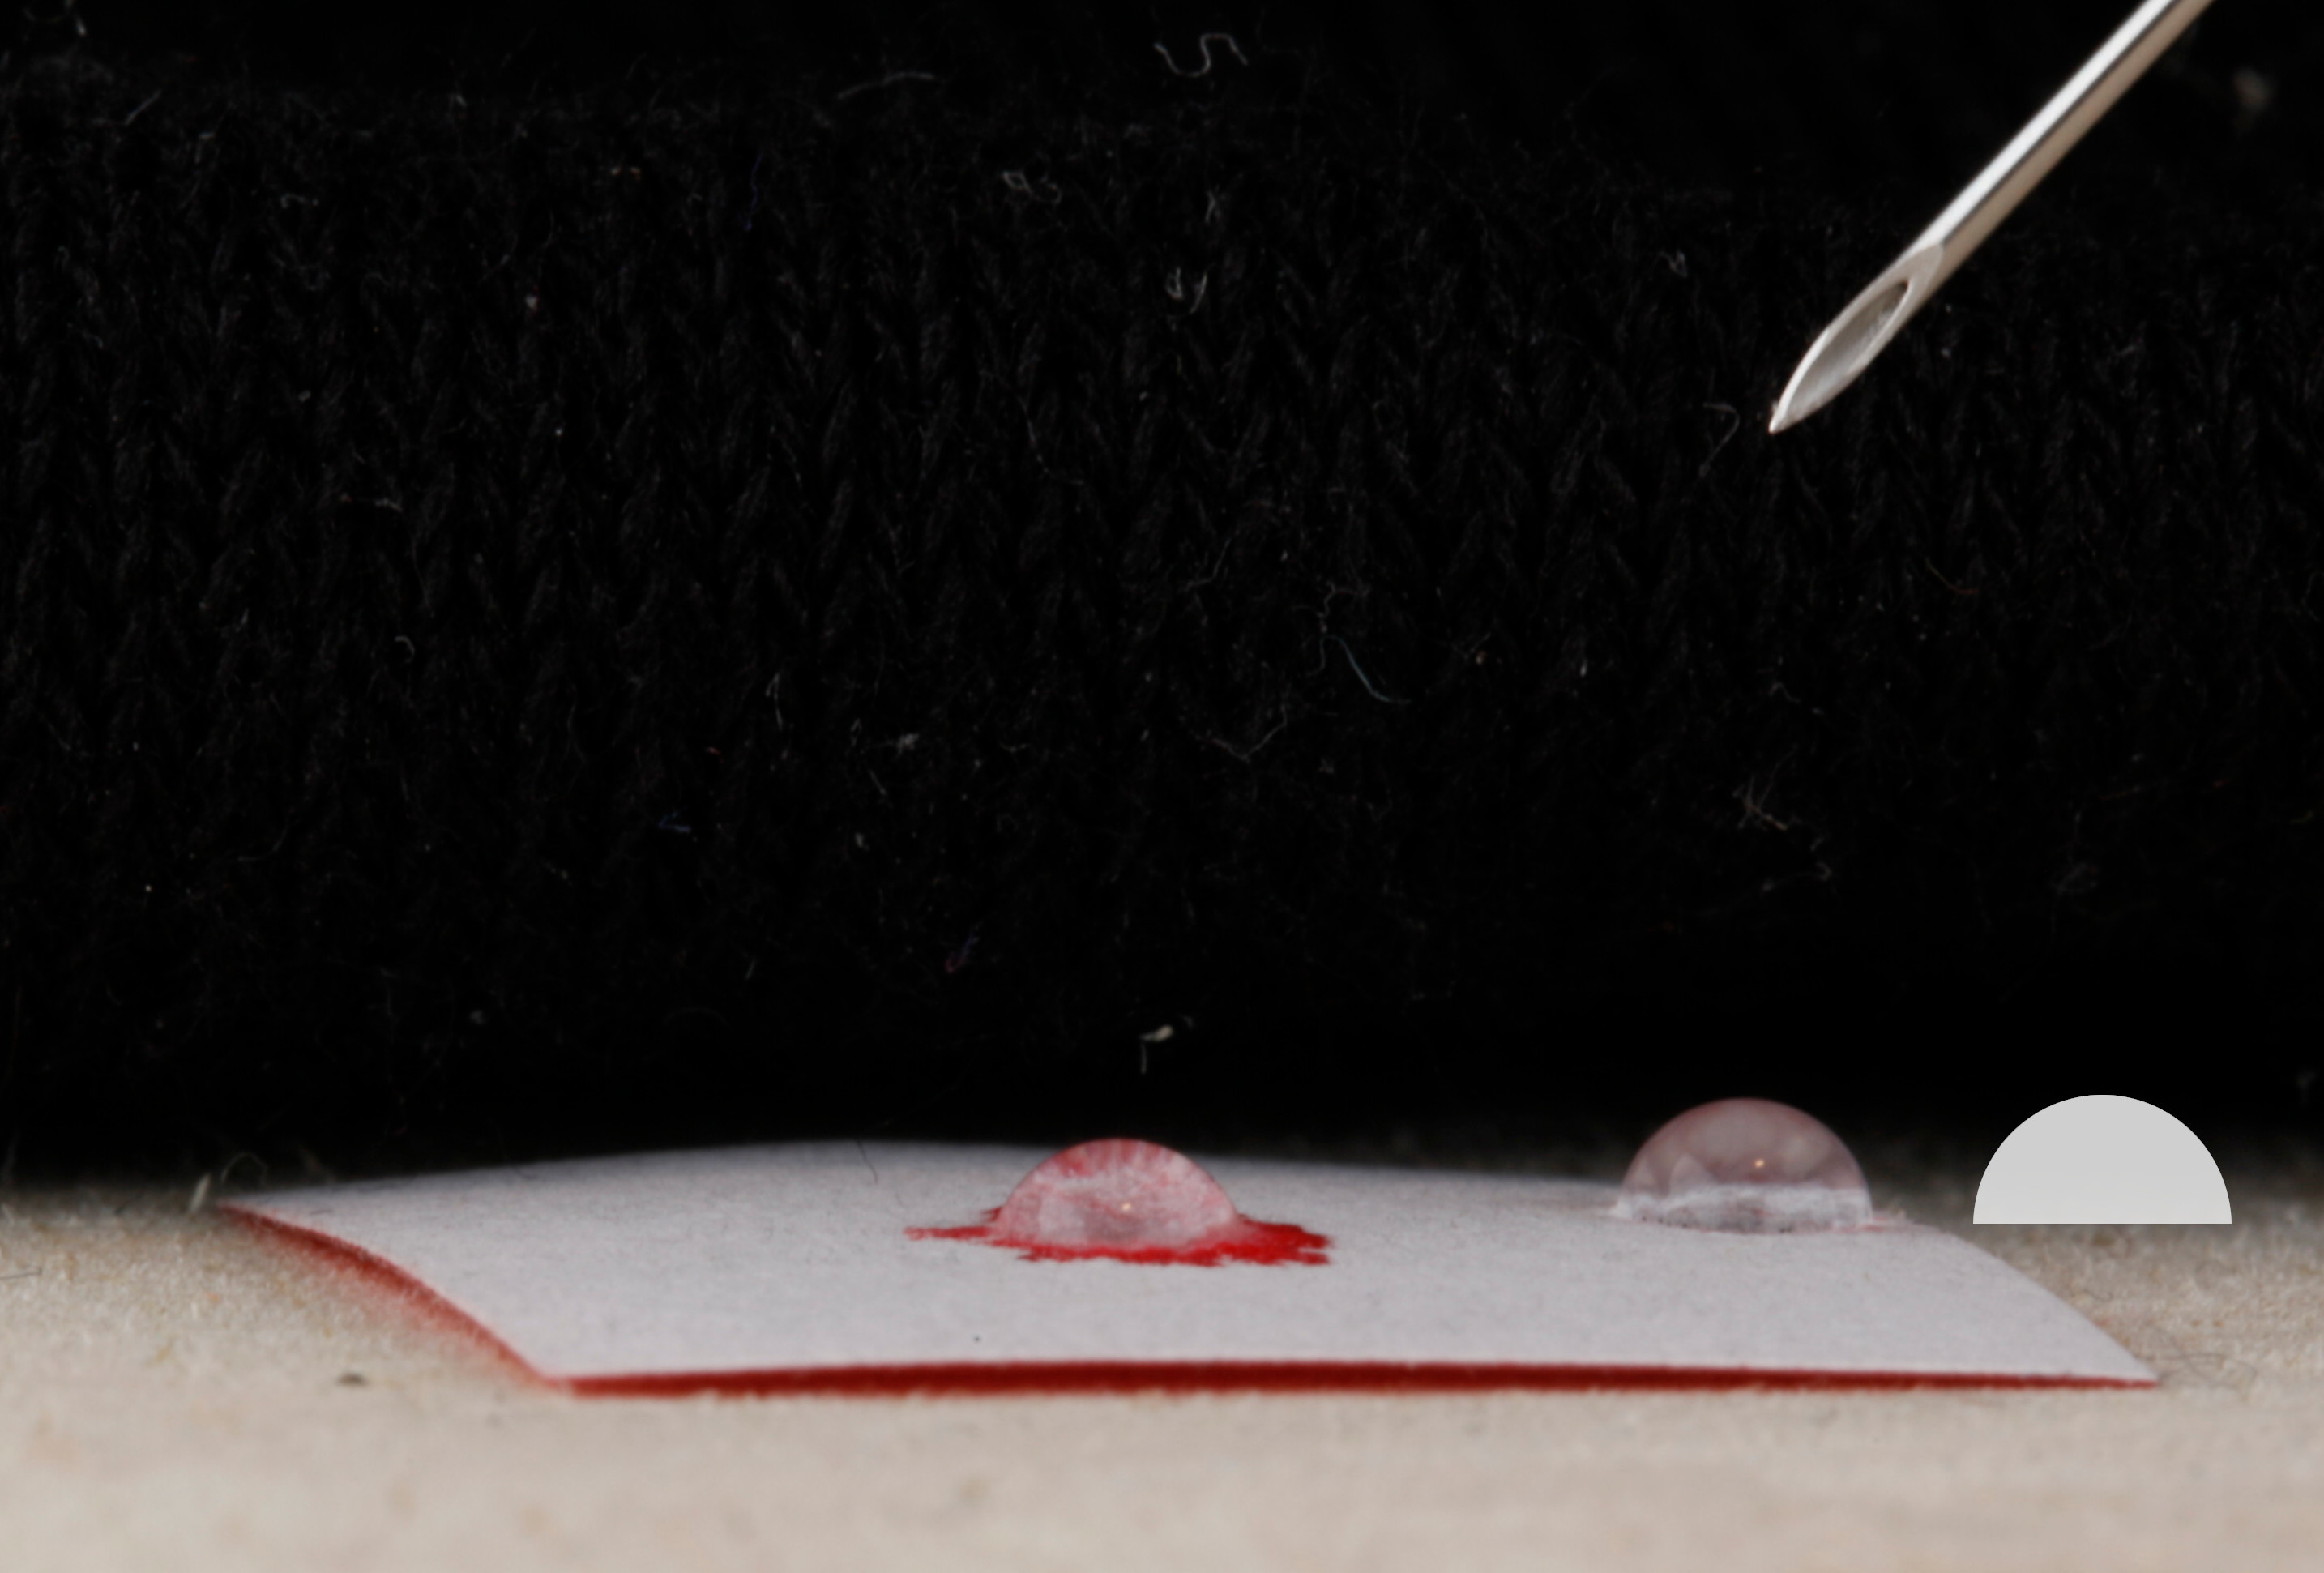
\includegraphics[width=0.8\textwidth]{Bilder/IMG_6683.JPG}
    \caption{Messung des Kontaktwinkels. Links ist ein Tropfen zu sehen, der mehrere Minuten auf dem Tape verweilt. Rechts ist ein neuer Wassertropfen, daneben noch der gefittete Kreis.} 
    \label{fig:winkTropf}
\end{figure}

Die Verfärbungen des Tapes sind abhängig von der Andruckdauer, Anpressdruck, der Geometrie des Schnees, dem Messablauf und dem LWC.

Bei einem ersten Feldversuch \ref{ersterFeldVer} konnten vielversprechende Ergebnisse gemessen werden.

\iffalse

Das 5559 Tape ist kostengünstig und zeigt innerhalb von weniger als 60 Sekunden das flüssige Wasser in einer Schicht an. Allerdings muss die Dichte des Schnees separat gemessen werden, da das Tape nur das flüssige Wasser anzeigt. Der Testaufbau beinhaltete das Kleben des 5559 Tapes auf ein rund 200 g schweres Objekt, das Freilegen einer neuen Schneeoberfläche mit einem Messer, das Auflegen des Tapes auf den Schnee und das Warten für 10, 30, 60 und 120 Sekunden. Anschließend wurde das Klebeband fotografiert und die rote gegen die weiße Fläche entweder optisch oder mithilfe von Python berechnet.

herkunft: Aus dem Elektronik bereich. zum beispiel in handys. wenn das tape rot geworden ist, ist wasser eingedrungen und der Hersteller kann eine garatieleistung ablehnen.

Funktionsweise: das papier basierte klebeband wird nass. die rote Farbe auf der Unterseite des Klebebands blutet durch das weisse obere Papier. die Roten Teile zeiget dann permanet wasser an.

Auswahl von 5559: der Hersteller 3M hat mehrere Produkte zu Water Indikator. 5559 zeichnet sich durch die dünnere Dicke und somit durch die schneller Anzeigegeschwindigkeit aus.

5559i ist auf einem transparenten substrat, was fraktisch für die optische auswertung wäre. Die Produkte sind in europa nur teilweise erhältlich. 3M verkauft nur Rollen mit 160 m. Zum testen wurde eine kleine rolle von einem Elektronikkomponenten Vertreiber gekauft.

Bei der Recherche zu LWC wurde keine verwendung von Water indicator tapes bemerkt. somit neuartig.

kostengünstig

zeitspanne pro messung weniger als 60 sek.

Dichte des Schnees muss seperat gemessen werden. 5559 zeigt nur das flüssige wasser in einer schicht an.

Testaufbau: 5559 auf etwas rund 200 g schweres kleben. neue Oberfläche von schnee mit Messer abschneiden/freilegen. 5559 auf schnee legen und 10, 30 60, 120 sek warten. foto von klebeband machen. mit python rote vs. weise fläche berechnen. oder nur optisch beurteilen.
\fi


\subsection{Voltcraft}
die gaphit sonden, zwischen denen die spanung aufgebaut und der wiederstand gemessen wird sind im messkopf zu gut geschützt. daher kann keine Messung gemacht werden wenn die Probe in schnee gedrückt wird.

Mögliche lösung: Verlängerung der Graphit proben

mit stahlplatten

Verbindung des Graphits mit der Platte: kleben oder konstant drückne oder verschrauben.

in gaphit spahnend zu arbeiten ist anspruchsvoll und dreckig.
konstant drücknen ist fehleranfällig
Kleben: herstellen von leitfähigem Klebstoff:

test graphitpluver: 66 \% gewichtsprozent Graphitpulver, 33 \% Ergo 7410 Epoxy Klebstoff

test Aluminiumpulver: 66 \% gewichtsprozent Aluminiumpulver, 33 \% Ergo 7410 Epoxy Klebstoff


Ergebniss: nach 24 h, sodass der ergo 7410 aushärten konnte.
Alle Klebestellen sind angeschliffen worden als oberflächenvorbereitung

Wiederstand zwischen Punkt A B 2.6 \ohm

wiederstand ziwschen Punkt A C 0.2 \ohm

Wiederstand zwischen Punkt A D keine verbindung

Mechanische stabilität von Test Aluminiumpluver nicht so gut

Ist es möglich auf die stahlplatte zu verzichten und die Verlängerung mit der Graphit Epoxy mischung zu machen?

zwisched die beiden grafit stäbe ist eine PAAM Platte geklebt. alle offenen stellen des Epoxy/grafits ist mit reinem epoxy überzogen um kriechspannungen durch wasser zu verhindern.

Arbeitsschutzt, erklären

Schnee ist wasser das vom Boden verdampft, sich dann in der Atmosspäre an einem Nukleus kondesiert oder resubliemiert und dann auf den Boden zurück fällt.

Im Alltag weiss man, dass man mit den Harrfön nicht in die Dusche gehen darf, da Wasser elektrisch leitend ist. Diese Schlussfolgerung ist nicht sehr prezise. denn reines Wasser ist nicht leitend, sonder die  Ione (Salze) die im 'normalen' Wasser gelöst sind. Auf sehr geringem Niveu ist auch reines Wasser leitend, da sich spontan  1*10 ^ 7 M  Hydroniumionen (H_3 O^+) bilden und den pH Wert 7 bilden.

Die Hypotese ist, dass sowohl die Verunreinigungen durch die Nuklei und die Hydroniuminonen genügend leitfägkeit bilden um einen Messwert im \mu S (Siemens = 1/\Ohm) Bereich zu messen.

Im Feldversuch konntekeine Leitfähigkeit gemessen werden.

EIne erweiterung dieser Messung ist, einen stoff zum schnee dazu zu geben, der gut leitfähig ist. dann wird der Versuchsaufbaumehr in die richtung \ref{} wo die Ausbreitung eines Stoffes im Schnee beobachtet wird. hier wäre diese beobachtung dann über die Leitfähigkeit und nicht wie in \ref{} optisch.


\subsection{Laser Refraktion und Reflezion}


\textbf{Funktionsweise}:

Mit einem Laser wird der Schnee sowohl durchleuchtet für die Refraktion als auch angeleuchtet für die Reflexion. In dem Abbildung \ref{fig:LaserHypothese} ist eine schematische Darstellung der Hypothese dargestellt. Die Grösse Wasseroberfläche und damit die Brennweite ändern sich je nach dem, wie viel Volumen Wasser auf den Eiskristallen ist. Die Effekte der Wasserlinsen sollten in der Refraktion sichtbar werden, indem sich helle und dunkle Bereiche bilden.




\begin{figure}
    \centering
    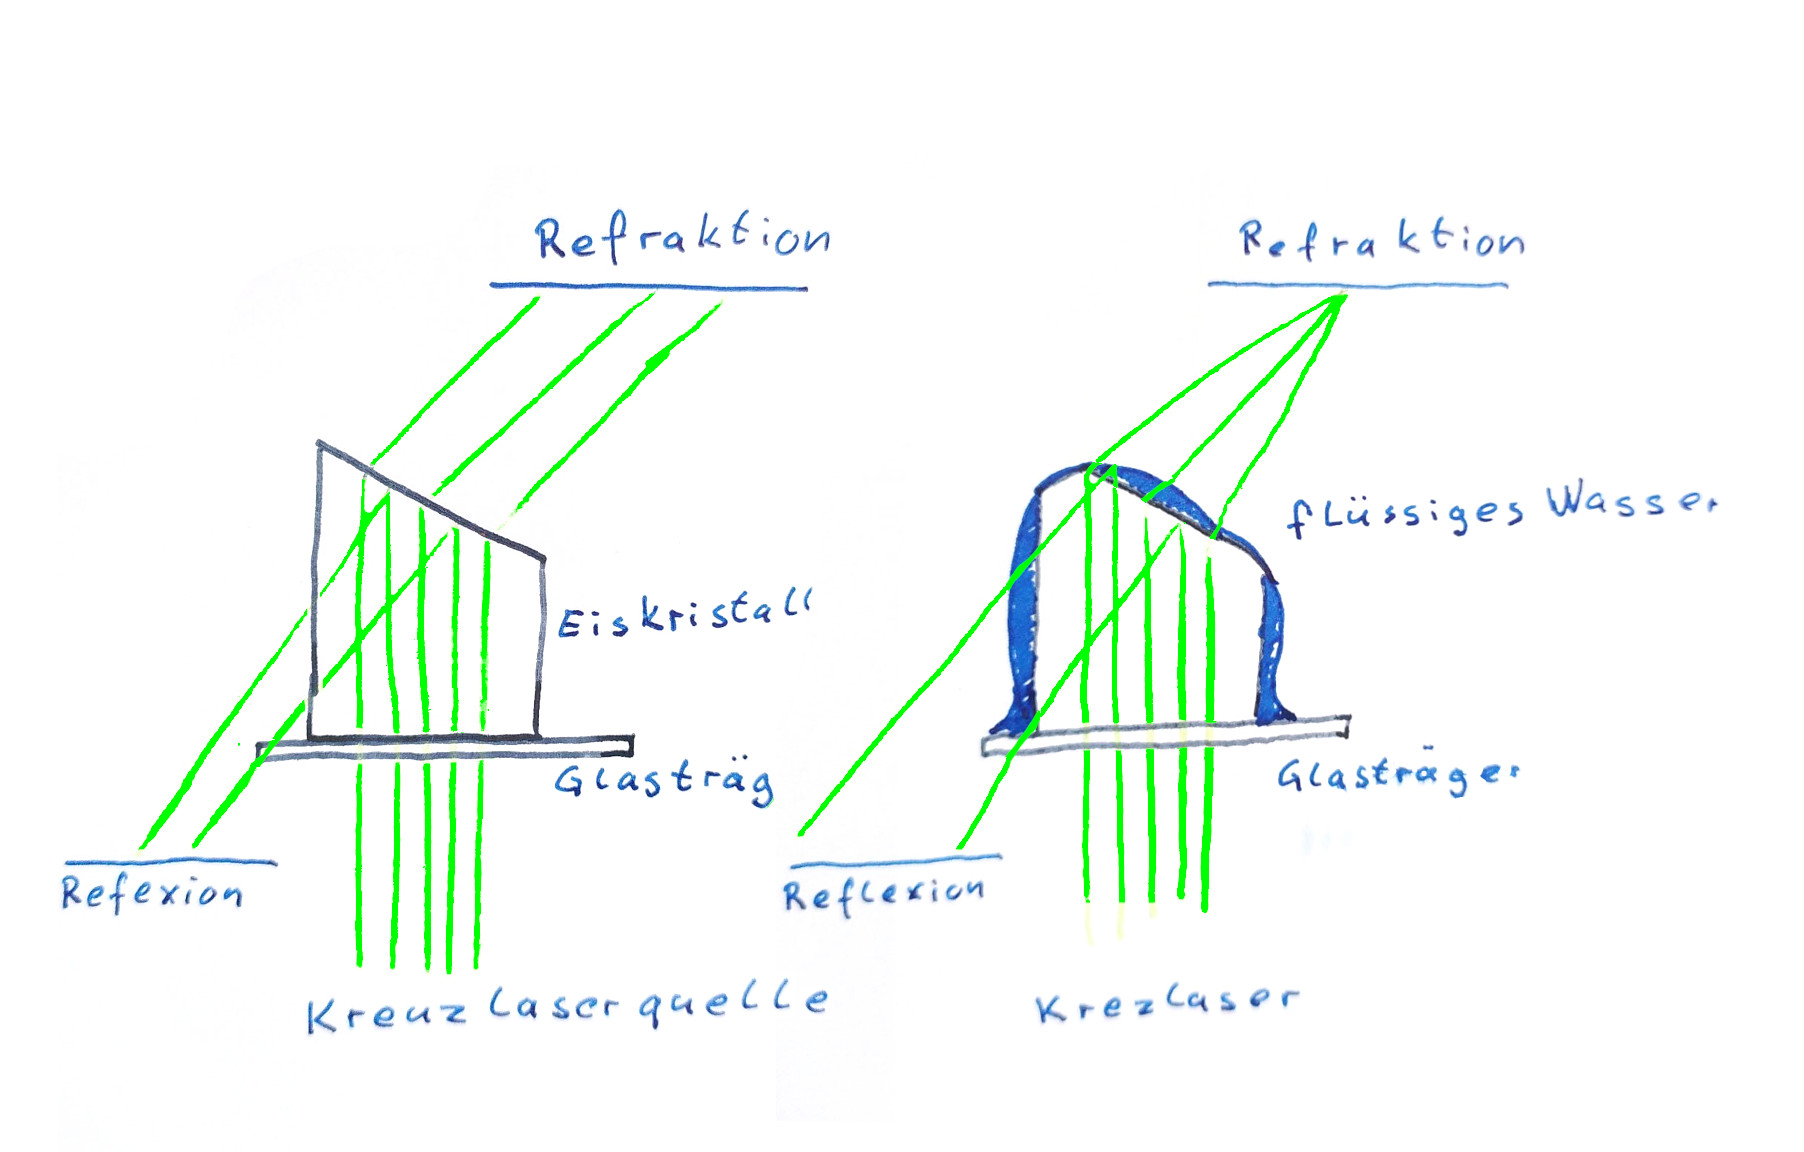
\includegraphics[width=0.8\textwidth]{Bilder/Reflaktion.jpeg}
    \caption{Hypothese wie das flüssige Wasser die optischen Eigenschaften der Eiskristalle beeinflusst}
    \label{fig:LaserHypothese}
\end{figure}

\textbf{Beispiele in anderen Sektoren}:

Refraktion wird in der Kristallografie angewendet. Die Reflexion von Wasser an einer Glasscheibe wird genutzt, um bei Autos Niederschlag auf der Windschutzscheibe zu messen.


\textbf{Benutzte Mittel für den Versuchsaufbau}:

Als Laserquelle wurde ein grüner Kreuzlaser (<5mW) genutzt. Um sowohl die Reflexion als auch die Refraktion gleichzeitig zu sehen, wurde die Schneeprobe auf einen Mikroskop-Objektträger platziert. Die Ergebnisse des Lasers wurden jeweils auf weissem Papier dargestellt. Die Refraktion wird auf dem Papier an der Unterseite der in Abbildung \ref{fig:LaserRef} zu sehende Holzplatte dargestellt. Mit einem Smartphone wurde eine Videoaufnahme gemacht, wie sich die Ergebnisse des Lasers verändern, während der Schnee schmilzt. Mit einem Spiegel wurde sowohl die Reflexion unten als auch die Refraktion oben gleichzeitig in einem Bild dargestellt.



In Abbildung \ref{fig:LaserAufbau} ist die Anordnung der verschiedenen Teile auf dem Stativmaterial zu sehen.


\begin{figure}
    \centering
    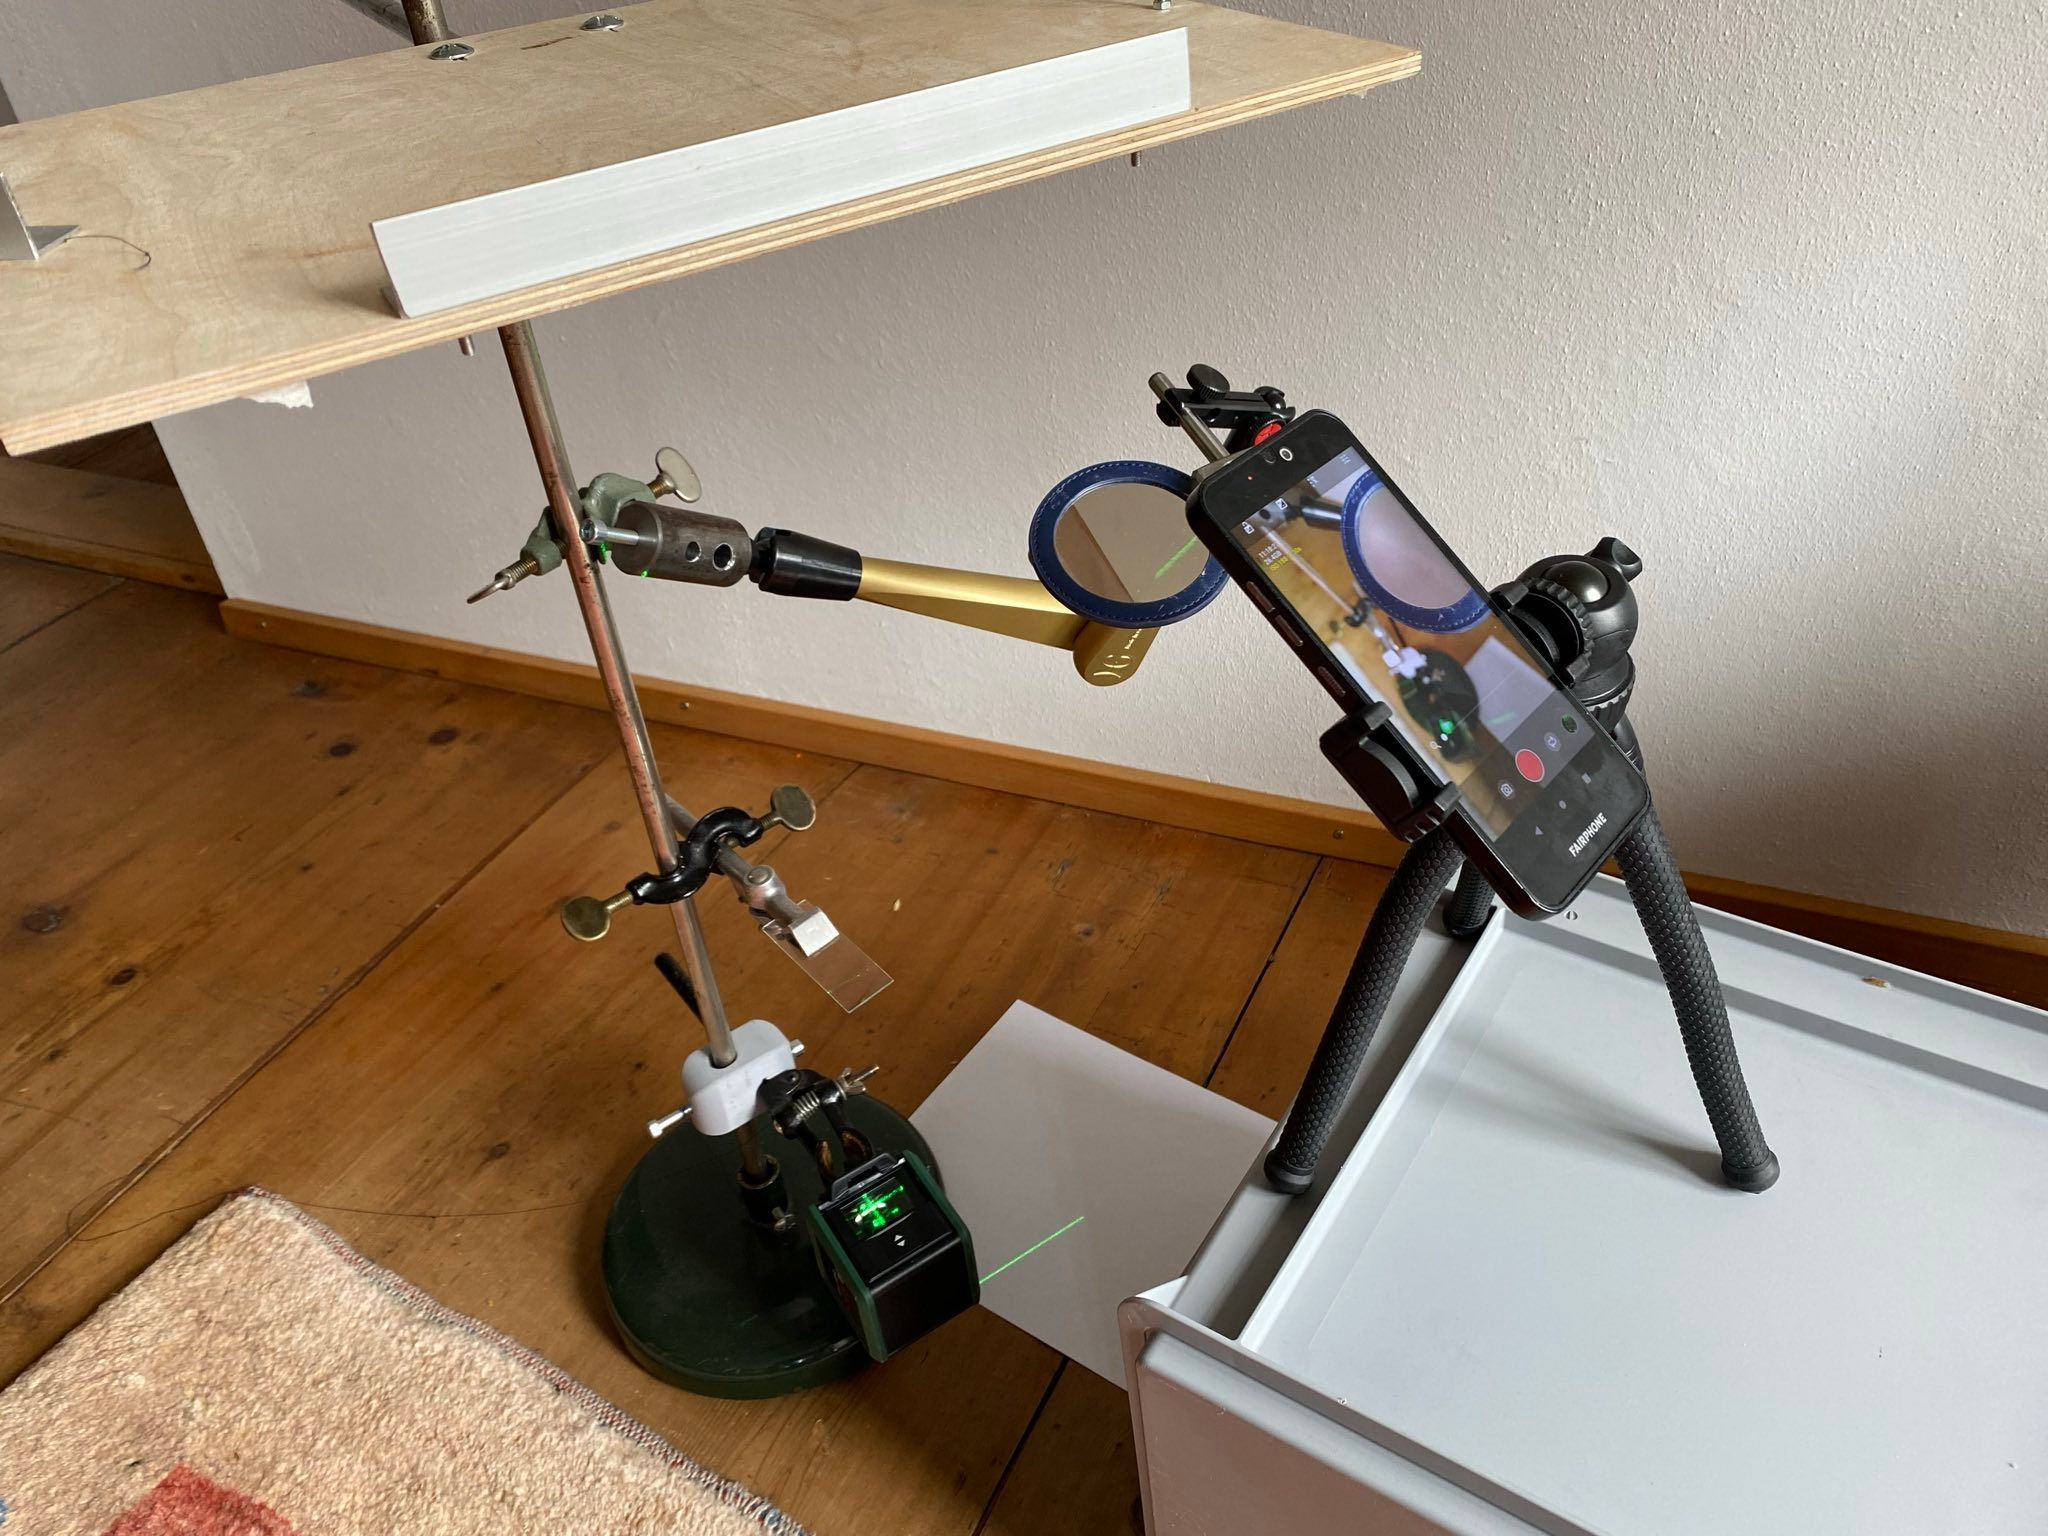
\includegraphics[width=0.8\textwidth]{Bilder/signal-2024-03-10-112013_006.jpeg}
    \caption{Versuchsaufbau der Laser Reflexion und Refraktion}
    \label{fig:LaserAufbau}
\end{figure}


\textbf{Funktionsweise des Versuchsaufbaus}:

Der Schnee wird im trockenen Zustand bei -10 Grad Celsius aus dem Gefrierschrank auf den gekühlten Objektträger gelegt. Dann wird beobachtet, wie sich die Ergebnisse ändern, wenn der Schnee an der Raumtemperatur schmilzt. Dieser Schmelzvorgang dauerte rund 3 Minuten. Dieser Aufbau ist suboptimal, denn die konstante Reflexion des Objektträgers muss aus dem Laserergebnis herausgerechnet werden.


\begin{figure}[H]
    \centering
    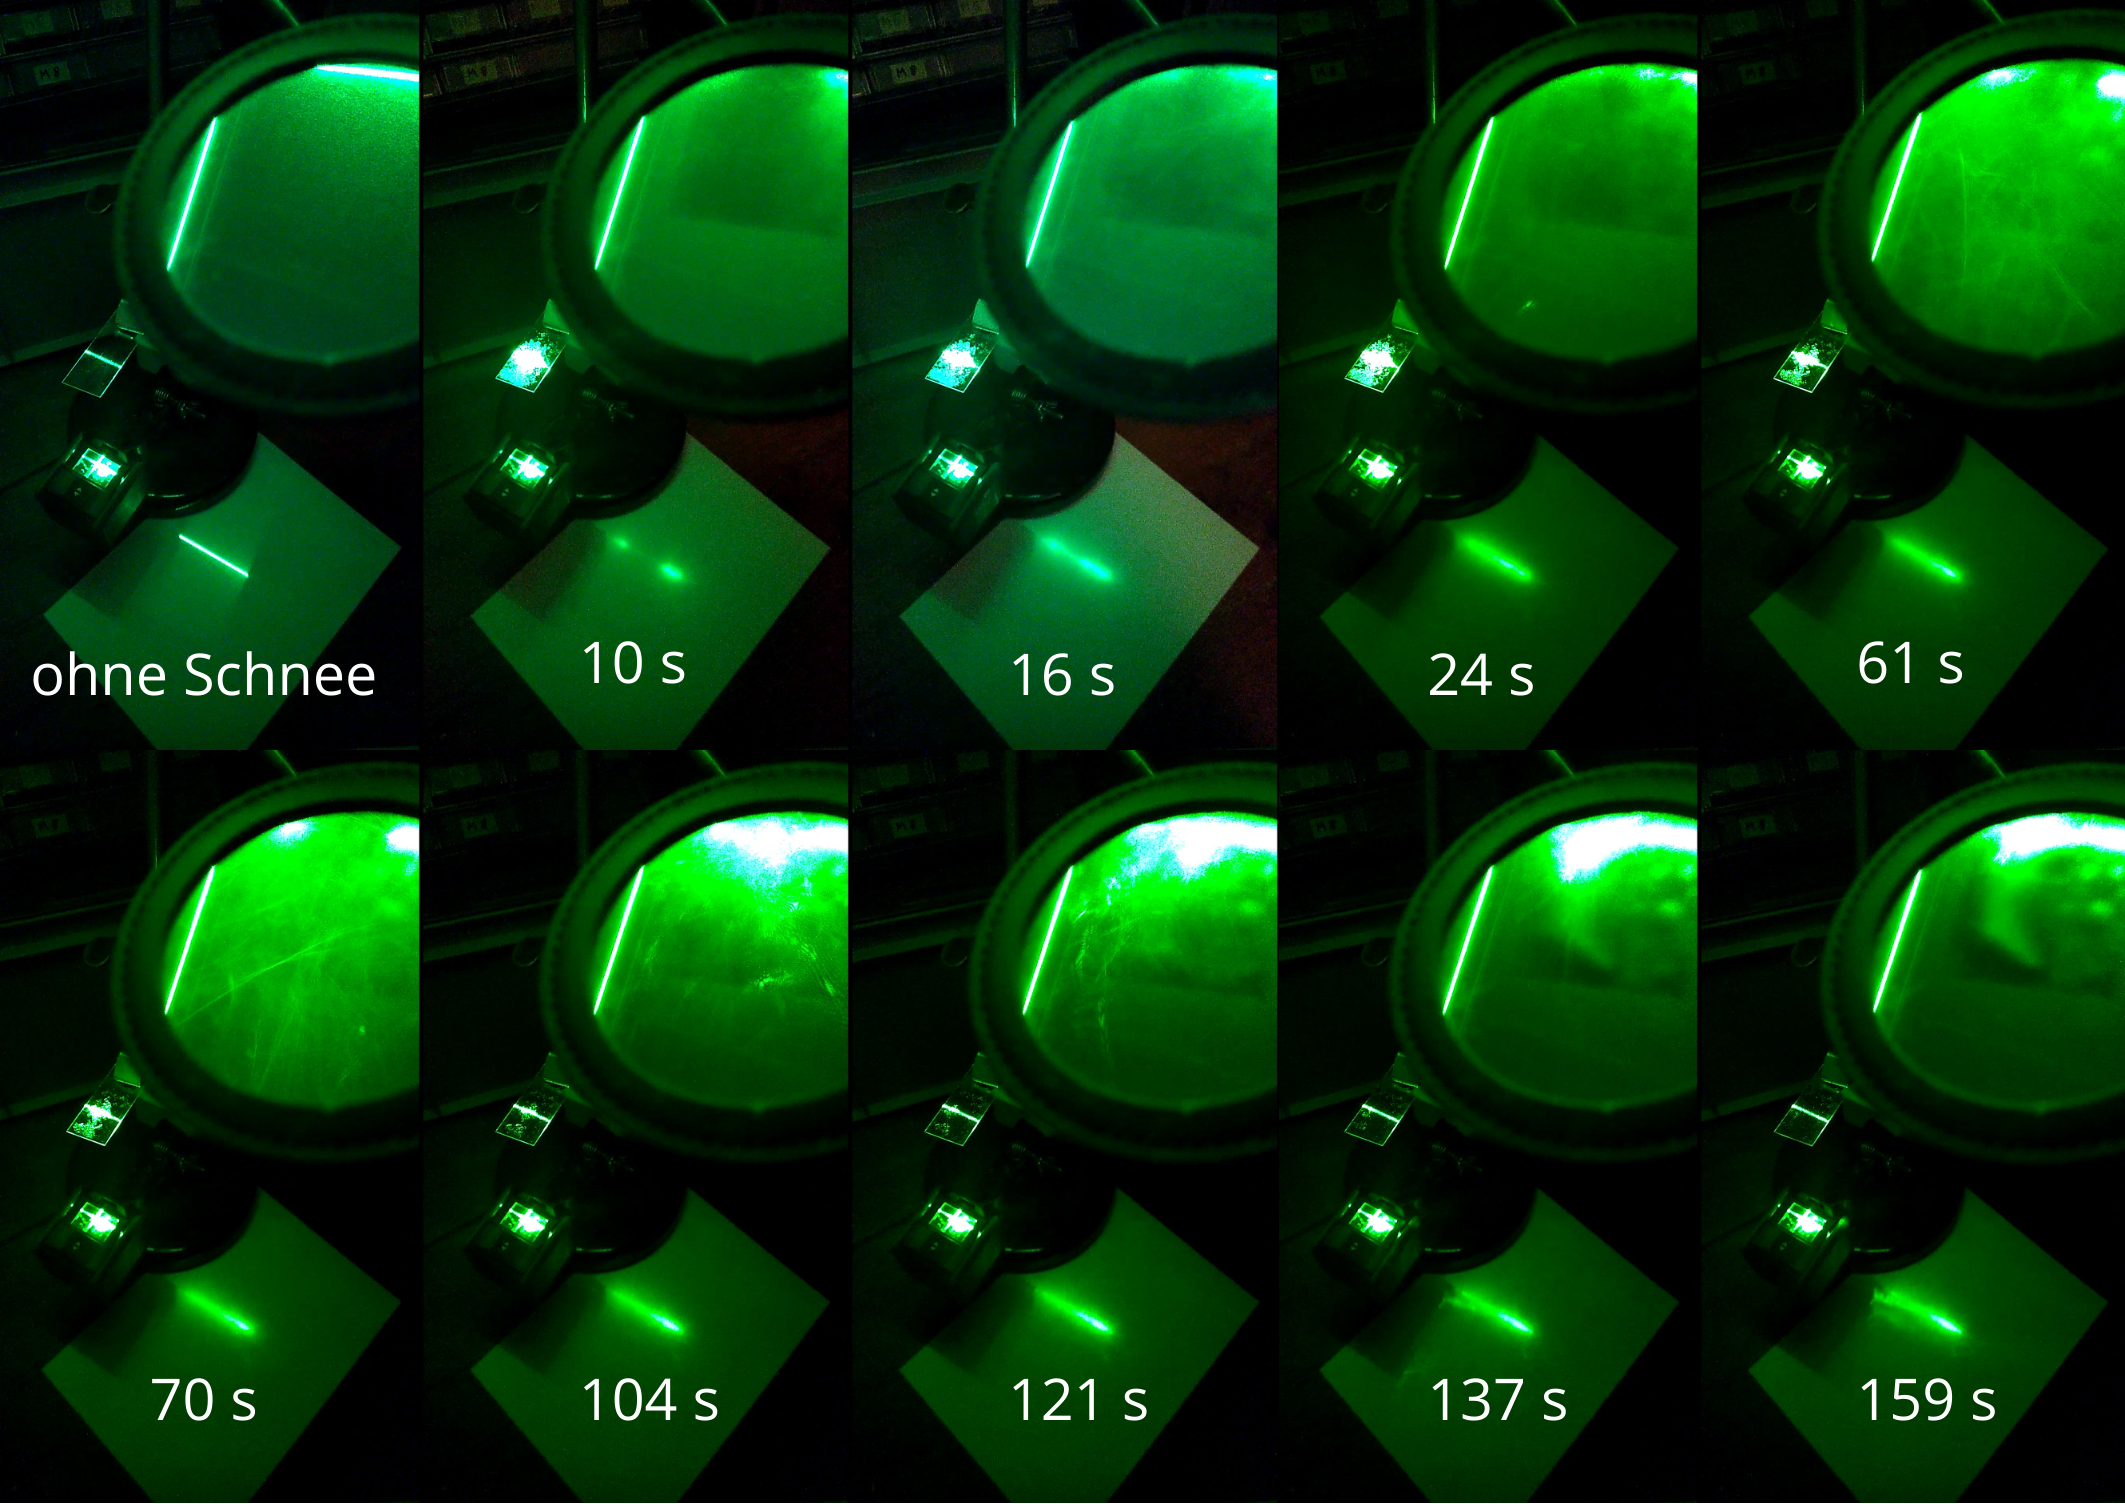
\includegraphics[width=0.8\textwidth]{Bilder/Screenshotfrom2024-04-0413-27-28.png}
    \caption{Messgrössen für die Reflexion und Refraktion, Veränderung über Zeit}
    \label{fig:LaserRef}
\end{figure}



\textbf{Messgrössen}:

Die Inhomogenität des Laserlichts und die Intensität können betrachtet werden. 



\textbf{Aussagekraft der Ergebnisse über den LWC}:

Die Ergebnisse werden direkt von Wasser beeinflusst. Um den Gewichts-LWC zu erhalten, ist aber die Geometrie der Eiskristalle von Bedeutung. Daher ist das Ergebnis nicht direkt in den LWC überführbar. Mit der 3D-Geometrie der Kristalle wäre die Aussagekraft höher.

\textbf{Reflexion zum Versuchsaufbau}:

Da zwei physikalische Messmethoden gleichzeitig getestet wurden, war der Versuchsaufbau nicht optimal für beide Messgrössen.

Mit den Ergebnissen der Refraktion bin ich zufrieden. Es ist eine klare Veränderung sichtbar, wenn der Schnee schmilzt.

Um vergleichbare Werte für den LWC zu bekommen, ist die Kristallgeometrie aber von Bedeutung. Die Messung der Geometrie übersteigt das Ausmass der BA.

Um die Messung der Refraktion durchzuführen, muss eine physikalisch unverändert Schneeprobe durchleuchtet werden. Dies stellt eine  Herausforderung dar, da der Schnee  aus der Schneedecke aufwendig extrahiert werden muss.

Das Ergebnis der Reflexion ist schwer zu beurteilen. In \cite{Donahue.2022} ist die Reflexion von EM-Wellen bereits mit Erfolg untersucht worden, in Abbildung \ref{fig:IRPaper} ist ein Ergebnis abgebildet.



\textbf{Verbesserungen des Versuchsaufbaus}:

Um bessere Reflexionsergebnisse zu bekommen, wäre es besser keinen Objektträger zu nutzen, sondern direkt auf den Schnee zu leuchten. Für eine statische Messung einer Schneeprobe muss die Luft um den Schnee herum gekühlt sein. Ein Ansatz dafür wird im Vorversuch \ref{sec:TinteVersuchsaufbau} umgesetzt. Mit dem Laser wird Energie in den Schnee eingebracht. Um das Schmelzen und damit Verfälschen des LWC zu minimieren, sollte ein möglichst schwacher Laser eingesetzt werden.




\subsection{Vibration}

Diese Hypothese geht davon aus, dass sich der Schnee bei mechanische Anregung von einem festen in den flüssigen Zustand übergeht. Je nach dem wie hoch der LWC ist, findet dieser Übergang statt oder nicht.

Um die Idee zu testen, wird ein vibrierendes Objekt mit hoher Dichte auf den Schnee gelegt, und es wird beobachtet, wie sich das Objekt durch den Schnee bewegt.

Die Form und Name des Objekts wurde vom AvaNode übernommen. Der Name  ist VibraNode. Für die Umsetzung wurde ein Morphologischer Kasten mit drei Varinanten erstellt.


\begin{figure}[H]
    \centering
    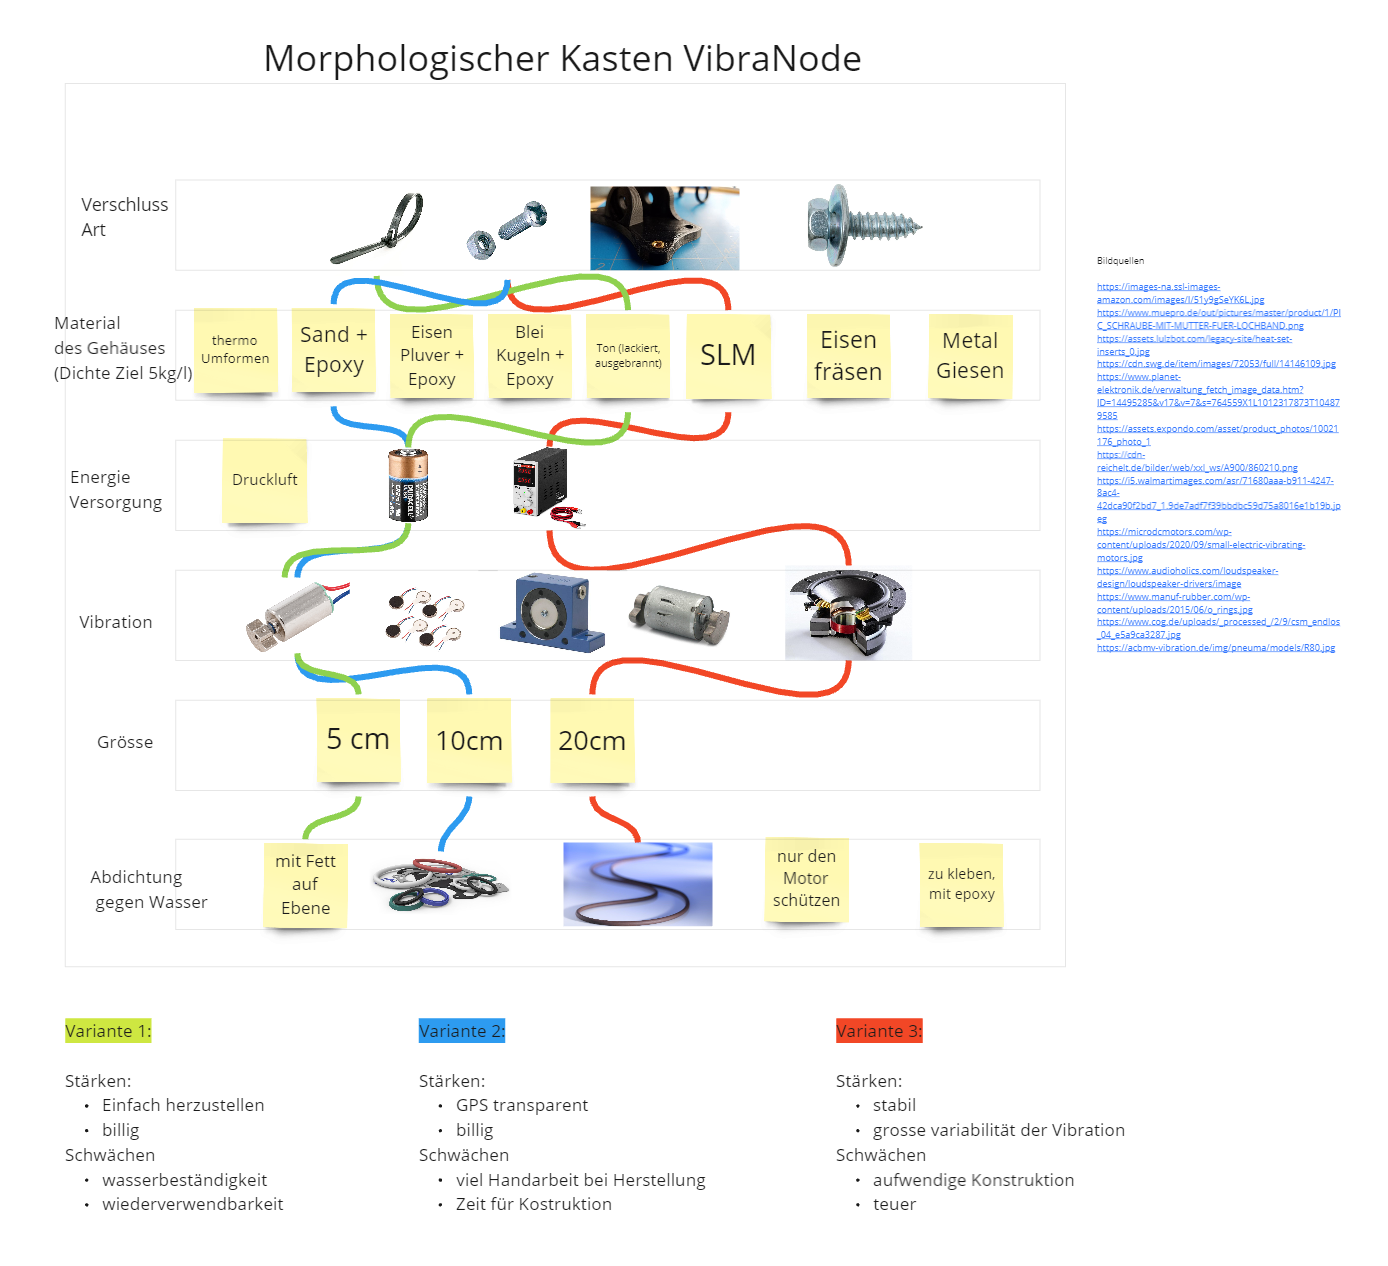
\includegraphics[width=0.9\textwidth]{Bilder/Unbenann2t.PNG}
    \caption{Morphologischer Kasten für VibraNode}
    \label{fig:Bildverarbeitnugskonzpet}
\end{figure}


Variante 1 wurde gewählt, da die Umsetztung und somit das Testen einfach ist. Die Schwächen, besonders die Wiederverwendbarkeit, sind hier in der Vorstudie noch nicht gravierend.

Die Testergebnisse fielen negativ aus. Der VibraNode konnte trotz seiner Dichte von 1600 kg/m3 nicht in den Schnee eindringen. Auch wenn der Schnee wurde mit flüssigem Wasser gesättigt war. Damit  stellt sich die neue Frage, ob der LWC einen kausalen oder nur einen korrelativen Zusammenhang mit Gleitschneelawinen hat, und wie weit die Vorgeschichte und andere Faktoren des Schnees mitbetrachtet werden muss. \cite{Altman.2015}


\subsection{Diffusion von Flüssigkeit}
\label{sec:TinteVersuchsaufbau}
Die Methode der Diffusion beobachtet, wie sich ein Stoff im Schnee ausbreitet. Für den Vorversuch wurde der Schnee unter ein Stereo-Mikroskop platziert. Der Versuch dauert etliche Minuten. Um zu verhindern, dass der Schnee von der warmen Raumluft aufgeschmolzen wird, ist der Schnee in einer Röhre aus Eis platziert. Während das -10 Grad Celsius kalte Eis langsam schmilzt, kann der Versuch durchgeführt werden. In der Abbildung \ref{fig:DiffMess} ist der Versuchaufbau dargestellt. Die Auswertung bei dem Vorversuch erfolgt visuell, indem beobachtet wird, wie sich blaue Tinte im Schnee ausbreitet.

Eine Kombination dieses Ansatzes mit der Leitfähigkeitsmessung (siehe \ref{sec:Volt}) ist möglich, wenn ein leitfähiger Stoff eingesetzt wird.

Ich vermute, dass dieser Ansatz von der Geometrie des Schnees beeinflusst wird. Der LWC ist wahrscheinlich weniger einflussreich als die Geometie der Eiskristalle.

\begin{figure}[H]
    \centering
    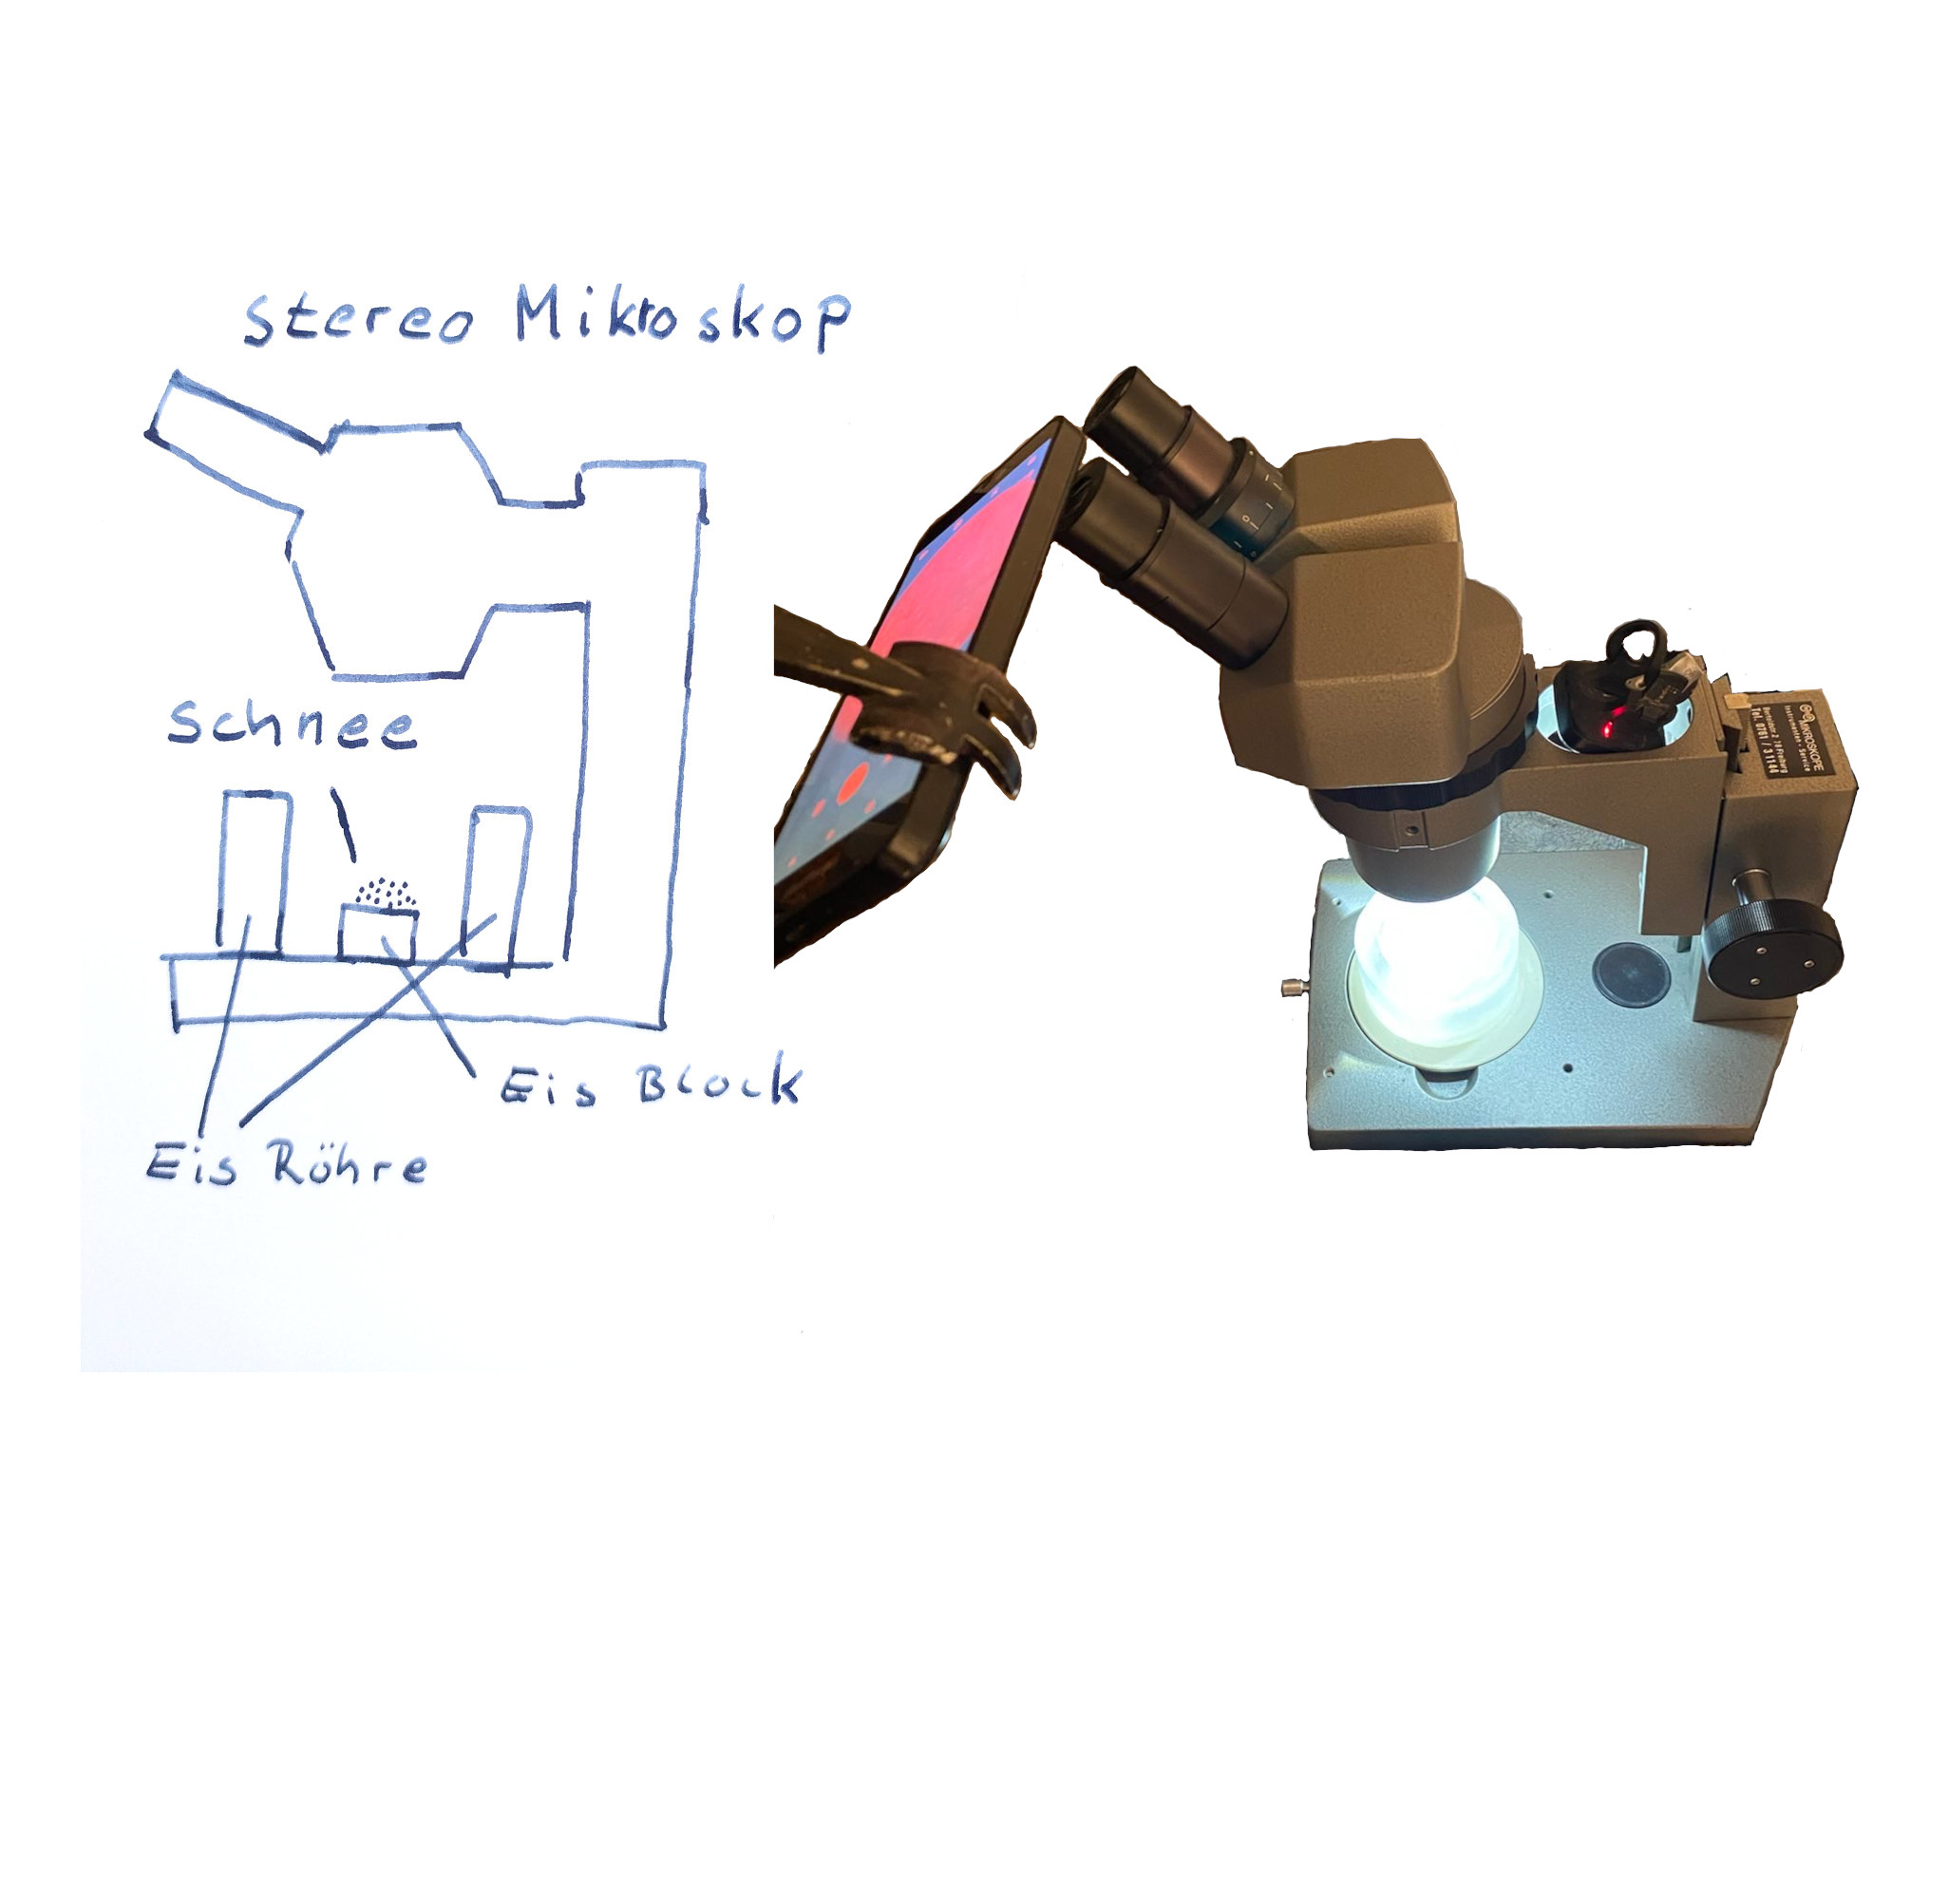
\includegraphics[width=0.8\textwidth]{Bilder/freistellen.jpeg}
    \caption{Aufbau einer Messung wobei der Schnee durch eine Eis Röhre gekühlt wird}
    \label{fig:DiffMess}
\end{figure}


\section{Funktionsmuster}

In diesem Kapitel werden die verschiedenen Funktionsmuster vorgestellt, die im Verlauf der Entwicklung entstanden sind. Ziel der Funktionsmuster war es, verschiedene Ansätze zur Messung und Auswertung des Flüssigwassergehalts (LWC) im Schnee zu erproben und zu optimieren. Jedes Funktionsmuster adressiert spezifische Herausforderungen und bringt neue Ideen ein, um die Messgenauigkeit und Benutzerfreundlichkeit zu verbessern. Anstatt jede Iteration im Detail zu beschreiben, werden hier die herausragenden Eigenschaften und innovativen Lösungen der einzelnen Entwicklungsstufen präsentiert. Dies soll einen Überblick über die Fortschritte und technischen Lösungen bieten, die im Laufe des Projekts entwickelt wurden.


\subsection{Agiles Hardware Devolopment}


Die Planung der Arbeit wird mit einem agilen Kanban-Board durchgeführt. Das heisst, es wird versucht, möglichst schnell zu einem Funktionsmuster zu kommen und daraus für die nächste Iteration zu lernen.

Um diese schnelle Arbeitsweise zu ermöglichen, habe ich folgende Reihenfolge zur Auswahl der Fertigungstechniken erstellt:

\begin{enumerate}
\item Bestehendes Objekt benutzen und modifizieren
\item Karton
\item IR-Lasercutter mit Sperrholz
\item 3D-Druck in FDM
\item Einkaufsteile bestellen
\item Selber fertigen (manuell drehen, fräsen, töpfern usw.)
\item Extern fertigen lassen
\end{enumerate}

Ein Endprodukt wird extern gefertigt werden müssen, um die Wertigkeit des Produkts an den Benutzer zu vermitteln. Die Seriengröße wird klein sein, da es wahrscheinlich kein Konsumerprodukt werden wird, sondern ein Forschungsinstrument bleibt.


\subsection{Messablauf}


Um an möglichst viele Schneetypen anwendbar zu sein, ist das Andrücken kraftgesteuert. In der Vorstudie \ref{sec:5559} war die Messung weggesteuert.

Als Kraft für den Anpressdruck wurde die Gewichtskraft gewählt. Es wird 80 \% der maximalen Traglast des Schnees für die Anpresskraft genutzt. So kann die Messung in Puderschnee bis hin zu Firn durchgeführt werden. Mit 36 g schweren Blechstücken kann das Gewicht zusammengesetzt werden. Das maximale Gewicht ist der maximal gemessene Wert der Traglast des Schnees im Feldversuch.

Die Messung wird wie folgt durchgeführt:

\begin{enumerate}
\item Einen Schnee finden, der möglichst homogen und von Menschen unbeeinflusst ist.
\item Mit einer Schaufel oder Ähnlichem wird ein kleiner Schneegraben schaufeln.
\item Auf der zu messenden Höhe eine saubere horizontale Fläche im Schnee mit der Blechklinge freilegen.
\item Das Stativmaterial wird im Schnee aufgebaut.
\item Mit der Federwaage oder durch Ausprobieren die maximale Traglast des Schnees ermitteln.
\item Die Gewichte der Tape-Halter zu 80 \% der maximalen Traglast des Schnees zusammenschrauben.
\item Die Tape-Halter aus den zweifach geschützten Beuteln entnehmen.
\item Die Tape-Halter mit den Gewichten zusammenstecken.
\item Mit dem Kältespray die Tapes runterkühlen 0 Grad.
\item Mit der Wärmebildkamera überprüfen, ob die Tapes die richtige Temperatur haben.
\item Die Tapes vorsichtig horinzontal auf den Schnee aufsetzen.
\item Mit dem magnetischen Halter die Gewichte an das Stativmaterial befestigen.
\item 120 Sekunden warten, sodass das Wasser aus dem Schnee auf das Tape übergehen kann.
\item Mit Druckluft allfällige Schneeflocken vom Tape entfernen.
\item 300 Sekunden warten, bis das Tape einen stabilen Zustand erreicht hat.
\item Die Tape-Halter in der Lichtbox befestigen.
\item Ein Bild der Tapes aufnehmen.
\end{enumerate}


\subsection{Bildverarbeitung}
Die Auswertung des Tapes kann auf zwei Arten erfolgen. Eine einfache Variante, die bei den Vorversuchen genutzt wird, besteht darin mit den eigenen Augen die Grösse und Verteilung des Rots auf dem Tape abzuschätzen.



Um dieses subjektive Schätzung durch eine objektive Quantifizierung zu ersetzen, wurde eine Pipeline zur digitalen Auswertung entwickelt. In einem ersten Schritt, illustriert in Abbildung \ref{fig:Bildverarbeitnugskonzpet}, wird die Fotografie eines Tape ausgewählt und in ein schwarz-weisses Bild übersetzt, so dass die vorher roten Farbflecken nun deutlicher erkannt werden können.

Um aus dem Bild quantitative Zahlen zu bekommen, werden die Flecken nun einzeln erfasst und in einer Datenback gespeichert. In der Datenbank können dann statistische Aussagen über die Verteilung, Grösse der Flächen, die Struktur und die prozentualen Flächenanteil gemacht werden.



\begin{figure}
    \centering
    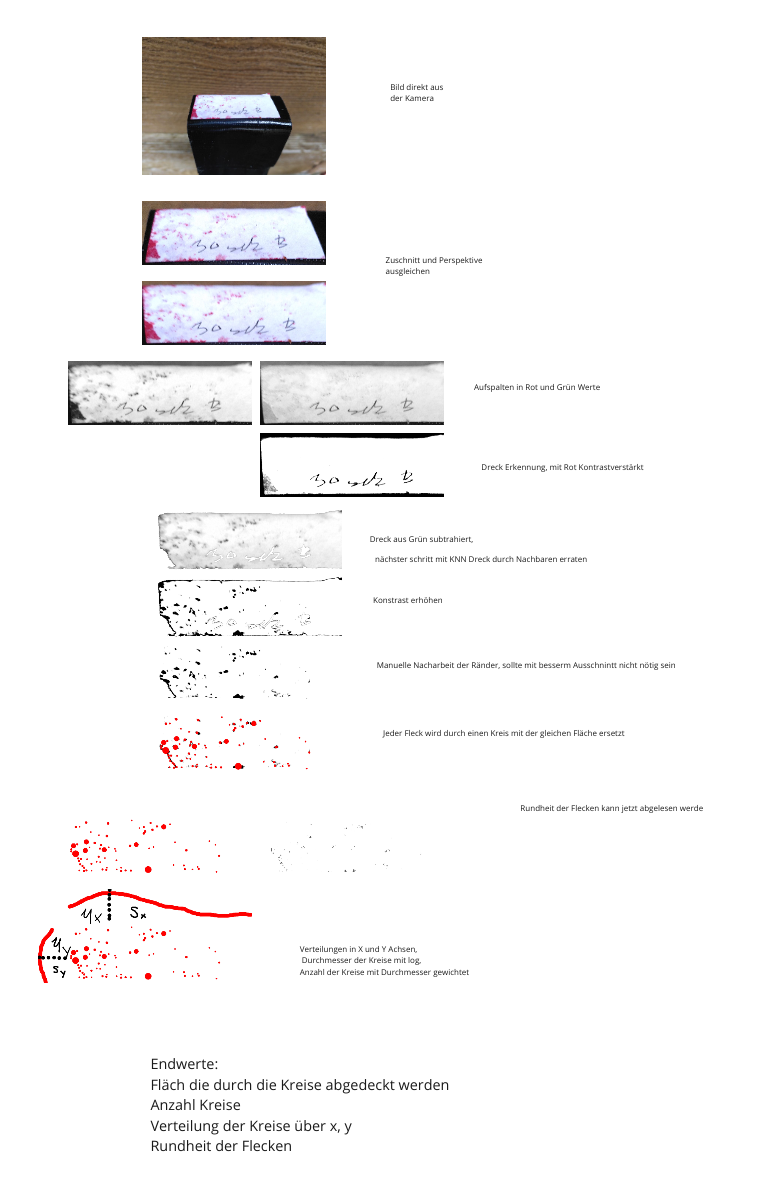
\includegraphics[width=0.9\textwidth]{Bilder/Screenshotfrom2024-04-0112-59-42.png}
    \caption{Bildverarbeitung Konzept}
    \label{fig:Bildverarbeitnugskonzpet}
\end{figure}

\newpage


\subsection{Extrahieren von Informationen aus Bilddaten}

Um aus den Bilddaten, die während Feldversuchen gesammelt werden, sinnvolle Erkenntnisse zu gewinnen, ist es entscheidend, die Daten effektiv zu strukturieren. Dazu wird eine Datenbank angelegt. Dies erleichtert die effiziente Speicherung und ermöglicht leistungsstarke Datenabfragefunktionen, wie z. B. das patter matching, die für eine umfassende Analyse wichtig sind.

Die im Feld gesammelten Daten werden zunächst in der Datenbank gespeichert und zu einem späteren Zeitpunkt analysiert.

Im Folgenden werden die Schritte zur Auslegung der Datenbank dargestellt. Der Code ist in Section \ref{sect:code} zu finden.

Die Methode wie die Datenbank hier ausgelegt wird, folgt der Vorlesung Datenbanksysteme 1. \cite{}

\subsubsection{Anforderungsanalyse}

Die Anforderungen ergeben sich aus der Funktionsweise des Messaufbaus.

Die Datenbank in dieser Bachelorarbeit wird relativ klein sein, da die Feldversuche zeitintensiv sind. Es wird vermutet, dass maximal 1000 Messungen mit jeweils 3 Taps und je 100 Kreisen durchgeführt werden.

Die Datenbank ist grösser angelegt, als sie für die Vorversuche in der Bachelorarbeit benötigt wird.

Es gibt vier Benutzer die mit der Datenbank interagieren. In der Grafik \ref{fig:user-db-entwurf} ist die schematische Darstellung.

\begin{figure}
    \centering
    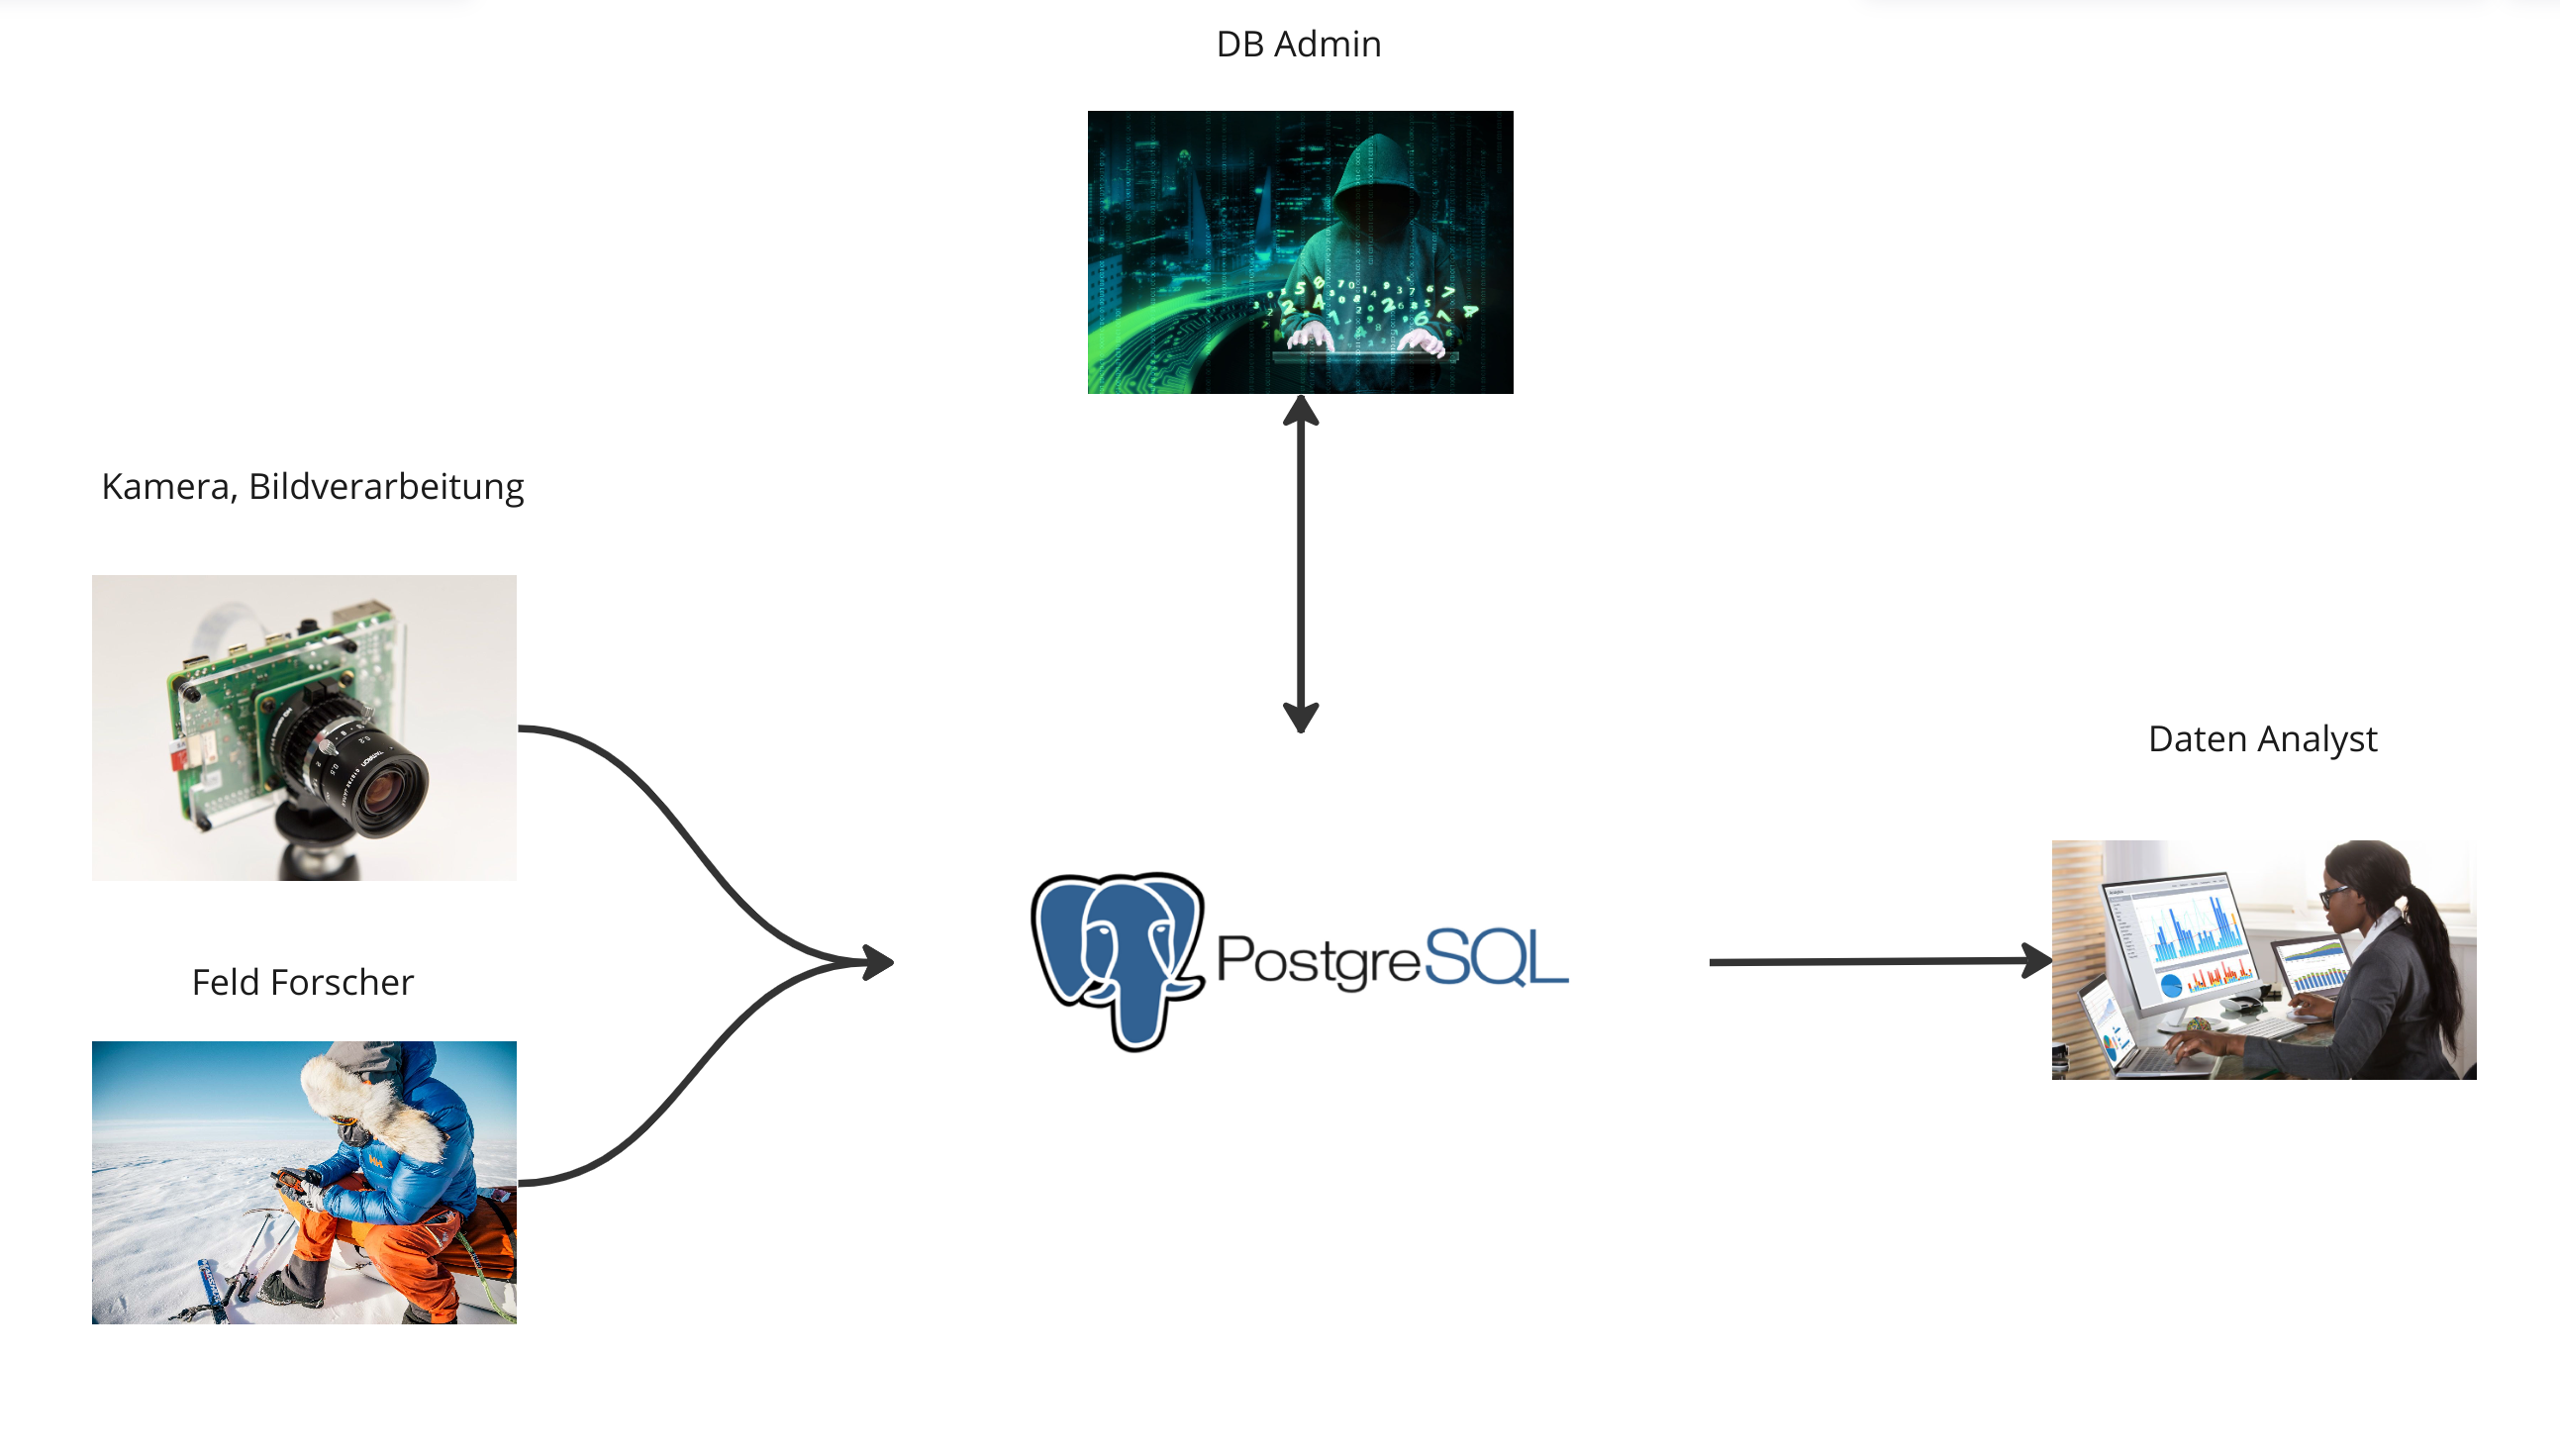
\includegraphics[width=0.8\textwidth]{Bilder/Screenshotfrom2024-04-0115-26-08.png}
    \caption{Benutzer der Datenbank}
    \label{fig:user-db-entwurf}
\end{figure}

\begin{enumerate}
\item Die Kamera, die die Bilder der Taps macht und auswertet, muss die Auswertungen in die Datenbank schreiben.
  \item Der Versuchsdurchführende gibt zusätzliche Informationen über den Versuch an, die er ebenfalls in die Datenbank schreiben muss.
    
    \item Der Analyst wird die Daten abfragen und hoffentlich Informationen daraus gewinnen.
    
    \item Der Datenbankadministrator wird im Normalbetrieb nicht benötigt, sollte jedoch berücksichtigt werden.
\end{enumerate}

Die Anforderungen an die Datenbank und ihre Benutzer werden entsprechend den Anforderungen des Messaufbaus und den Bedürfnissen der Benutzer festgelegt.

\ref{code:User}

\subsubsection{Konzeptueller DB Entwurf}

Mit der Unified Modeling Language (UML) wird in  \ref{fig:uml-db-entwurf} die Struktur der Datenbank dargestellt. Diese Darstellung ist noch lösungsunabhängig.

\begin{figure}
    \centering
    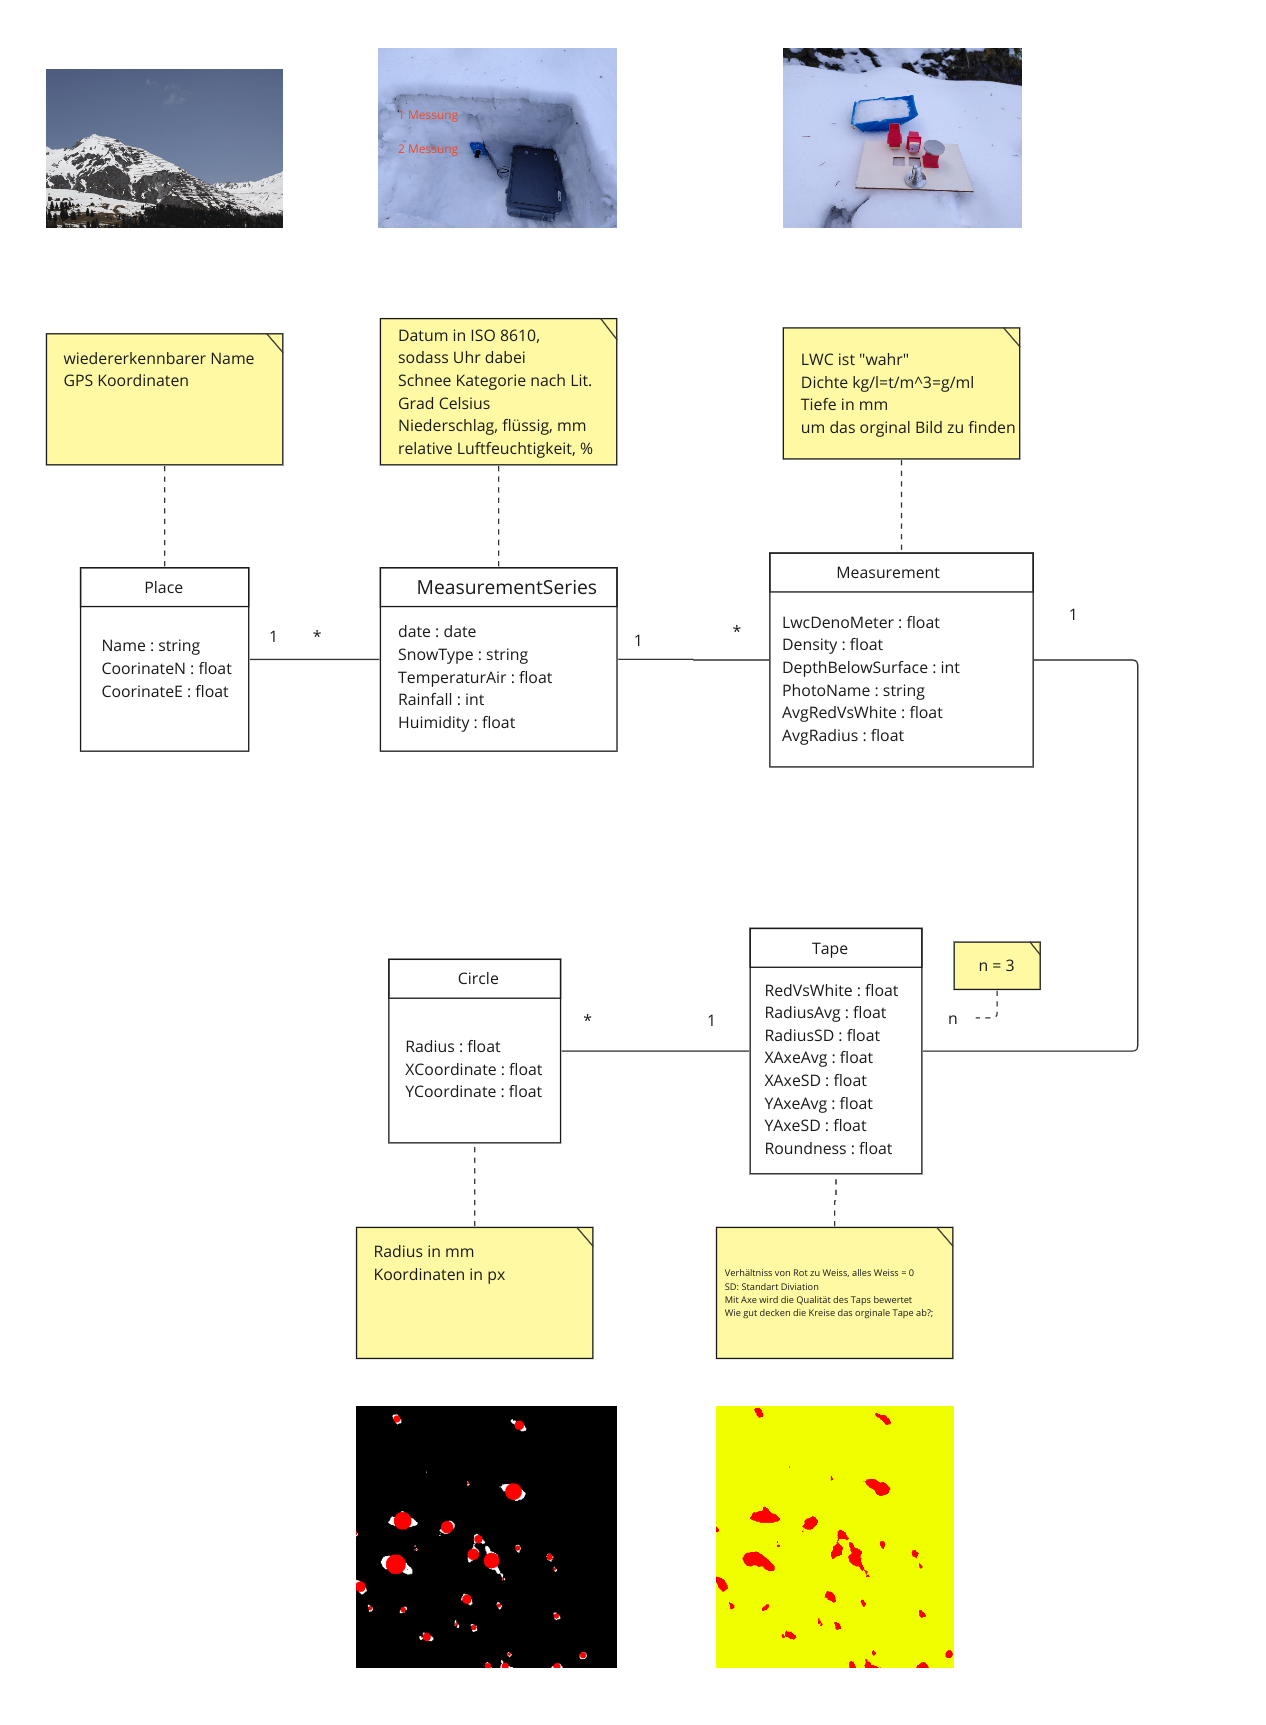
\includegraphics[width=0.8\textwidth]{Bilder/Screenshotfrom2024-04-1418-05-35.png}
    \caption{UML-Diagramm des konzeptuellen DB-Entwurfs}
    \label{fig:uml-db-entwurf}
\end{figure}



\subsubsection{Logischer DB Entwurf}


Um die Datenbank zu implementieren, wurde PostgreSQL gewählt. Es ist ein Free und Open-Source-System, das neue Features wie zum Beispiel JSON-Datentypen unterstützt.

Der folgende SQL-Code initialisiert die Datenbank: \ref{code:DBIni}

\subsubsection{Views für den Analysten}
Das Endziel besteht darin, eine Regression aus den Messungen und Taps zu erstellen, um den 'LWC Denoth' zu bestimmen. Für diese Aufgabe sind höchstwahrscheinlich nur bestimmte Angaben aus der Datenbank erforderlich.

Hier werden zwei Views erstellt: Der erste ist ein minimalistischer Ansatz, mit dem direkt weitergearbeitet werden kann. Der zweite View dient dazu, genauer zu verstehen, was in dem ersten View dargestellt ist.

Da die Ansichten für den read only Analysten bestimmt sind, muss keine aktualisierbarer View erstellt werden.

\ref{code:ViewDB}

\subsubsection{Physischer Entwurf}
Für die Beispieldaten wurden Daten aus der Vorstudie \ref{} für eine Messung verwendet.

Die Datenbank wird anfangs viele NULL-Werte enthalten, da beispielsweise die Wetterdaten nicht von einer API gefüllt werden.

Die Transaktionen sind in dieser Anwendung unproblematisch, da der Benutzer, der die Inserts durchführt (Raspberry, Feldforscher), zu einem früheren Zeitpunkt arbeitet als der Analyst.

Falls die Datenbank von meinem Laptop auf einen Server ausgelagert wird, werden die folgenden Tools zur Sicherheitsprüfung verwendet: \href{https://www.owasp.org}{www.owasp.org} und \href{http://sqlmap.org/}{http://sqlmap.org/}.

\subsubsection{Python-Interaktion mit der Datenbank}

Für die Interaktion mit der Datenbank werden verschiedene Python-Skripte verwendet, die je nach Benutzer unterschiedliche Aufgaben erfüllen.

Das folgende Python-Skript ist dazu da Bilder von Taps zu analysieren und die daraus gewonnenen Daten in die Datenbank einzufügen. \ref{code:RaspKam}

Das nächste Python-Skript wird interaktiv vom Versuchsleiter verwendet. Zur Zeit ruft das Skript auch noch die Bildanalyse auf. \ref{code:FeldUser}


\subsubsection{Nächste Schritte}

Die Python-Programme sollten weiterentwickelt werden, um sämtliche verfügbaren Daten in der Datenbank zu nutzen und um die Funktionalität zu verbessern.

Aktuell läuft die Datenbank mit dem Benutzer Postgres auf einem Laptop. Eine Auslagerung auf einen Server ist derzeit keine Priorität, da dies mit Sicherheitsrisiken verbunden ist. Das Hauptziel dieser Produktentwicklungs Bachelorarbeit besteht darin, das Verhalten des Taps zu verstehen. Sobald dieses Ziel erreicht ist, können weitere Schritte zur Optimierung und Sicherung der Datenbankinfrastruktur unternommen werden.

Sobald die Feldversuche durchgeführt worden sind, wird sich die DB an die tatzächlie Nutztung noch anpassen.



\subsection{Testkriterien}
\input{TestKrit.tex}

\subsection{Wiederstand gegen Umwelteinflüsse}

 Um zu verhindern, dass das Tape den Schnee anschmilzt und die Werte verfälscht, muss das Tape mit einem Kältemittel gekühlt werden. Daher ist es wichtig abzuklären. wie das Tape auf chemische Stoffe und thermische Veränderungen reagiert.

Chemisch getestet wurden zuerst Isopropanol, Nitroverdünner und Aceton.  Das Tape verfärbte sich temporär. Nachdem das Lösungsmittel abgedampft war, konnten keine Veränderung am Tape mehr festgestellt werden. Wenn das Tape nun jedoch mit Wasser aktiviert wurde, konnte beobachtet werden, dass die vorbehandelten Bereiche stärker auf Feuchtigkeit  reagierten. 


Die Kältemittel aus \ref{sec:Mess} haben ebenfalls das Tape temporär verfärbt. Hier wurde keine Veränderung der Wasseranzeige beobachtet.

Die Reaktionsfähigkeit des Tapes wurde bei -10 Grad getestet.

Zusätlich wurden auch die thermischen Eigenschaften bei Wärmeeinwirkung getestet. Bei Wärmeeinwirkung mit einer Heissluftpistole hat sich zum einen der Klebstoff gelöst und das weisse Papier des Tapes wurde braun. Die Bereiche des Tapes, die nach dem abkühlen noch weiss waren, haben auf Wasser noch immer gut reagiert. Die Braun verfärbte Teile konnten kein Wasser mehr anzeigen. Die Hitzeentwicklung beispielsweise durch die Lagerung des Tapes in einem Fahrzeug, das in der Sonne steht, sind aber deutlich niedriger.

Der Temperatureinsatzbereich ist vom Hersteller als - 40 bis 121 Grad Celsius angegeben.


\subsection{Ergebnisse der Versuche}



\textbf{Erster Feldversuch}
\label{ersterFeldVer}

Im ersten Versuch wurde untersucht, wie sich die Andruckzeit des Tapes auf das Messergebnis auswirkt. Bereits nach 5 Sekunden war ein Ergebnis messbar, welches bei 120 Sekunden ausgeprägter wurde.

\begin{figure}[H]
    \centering
    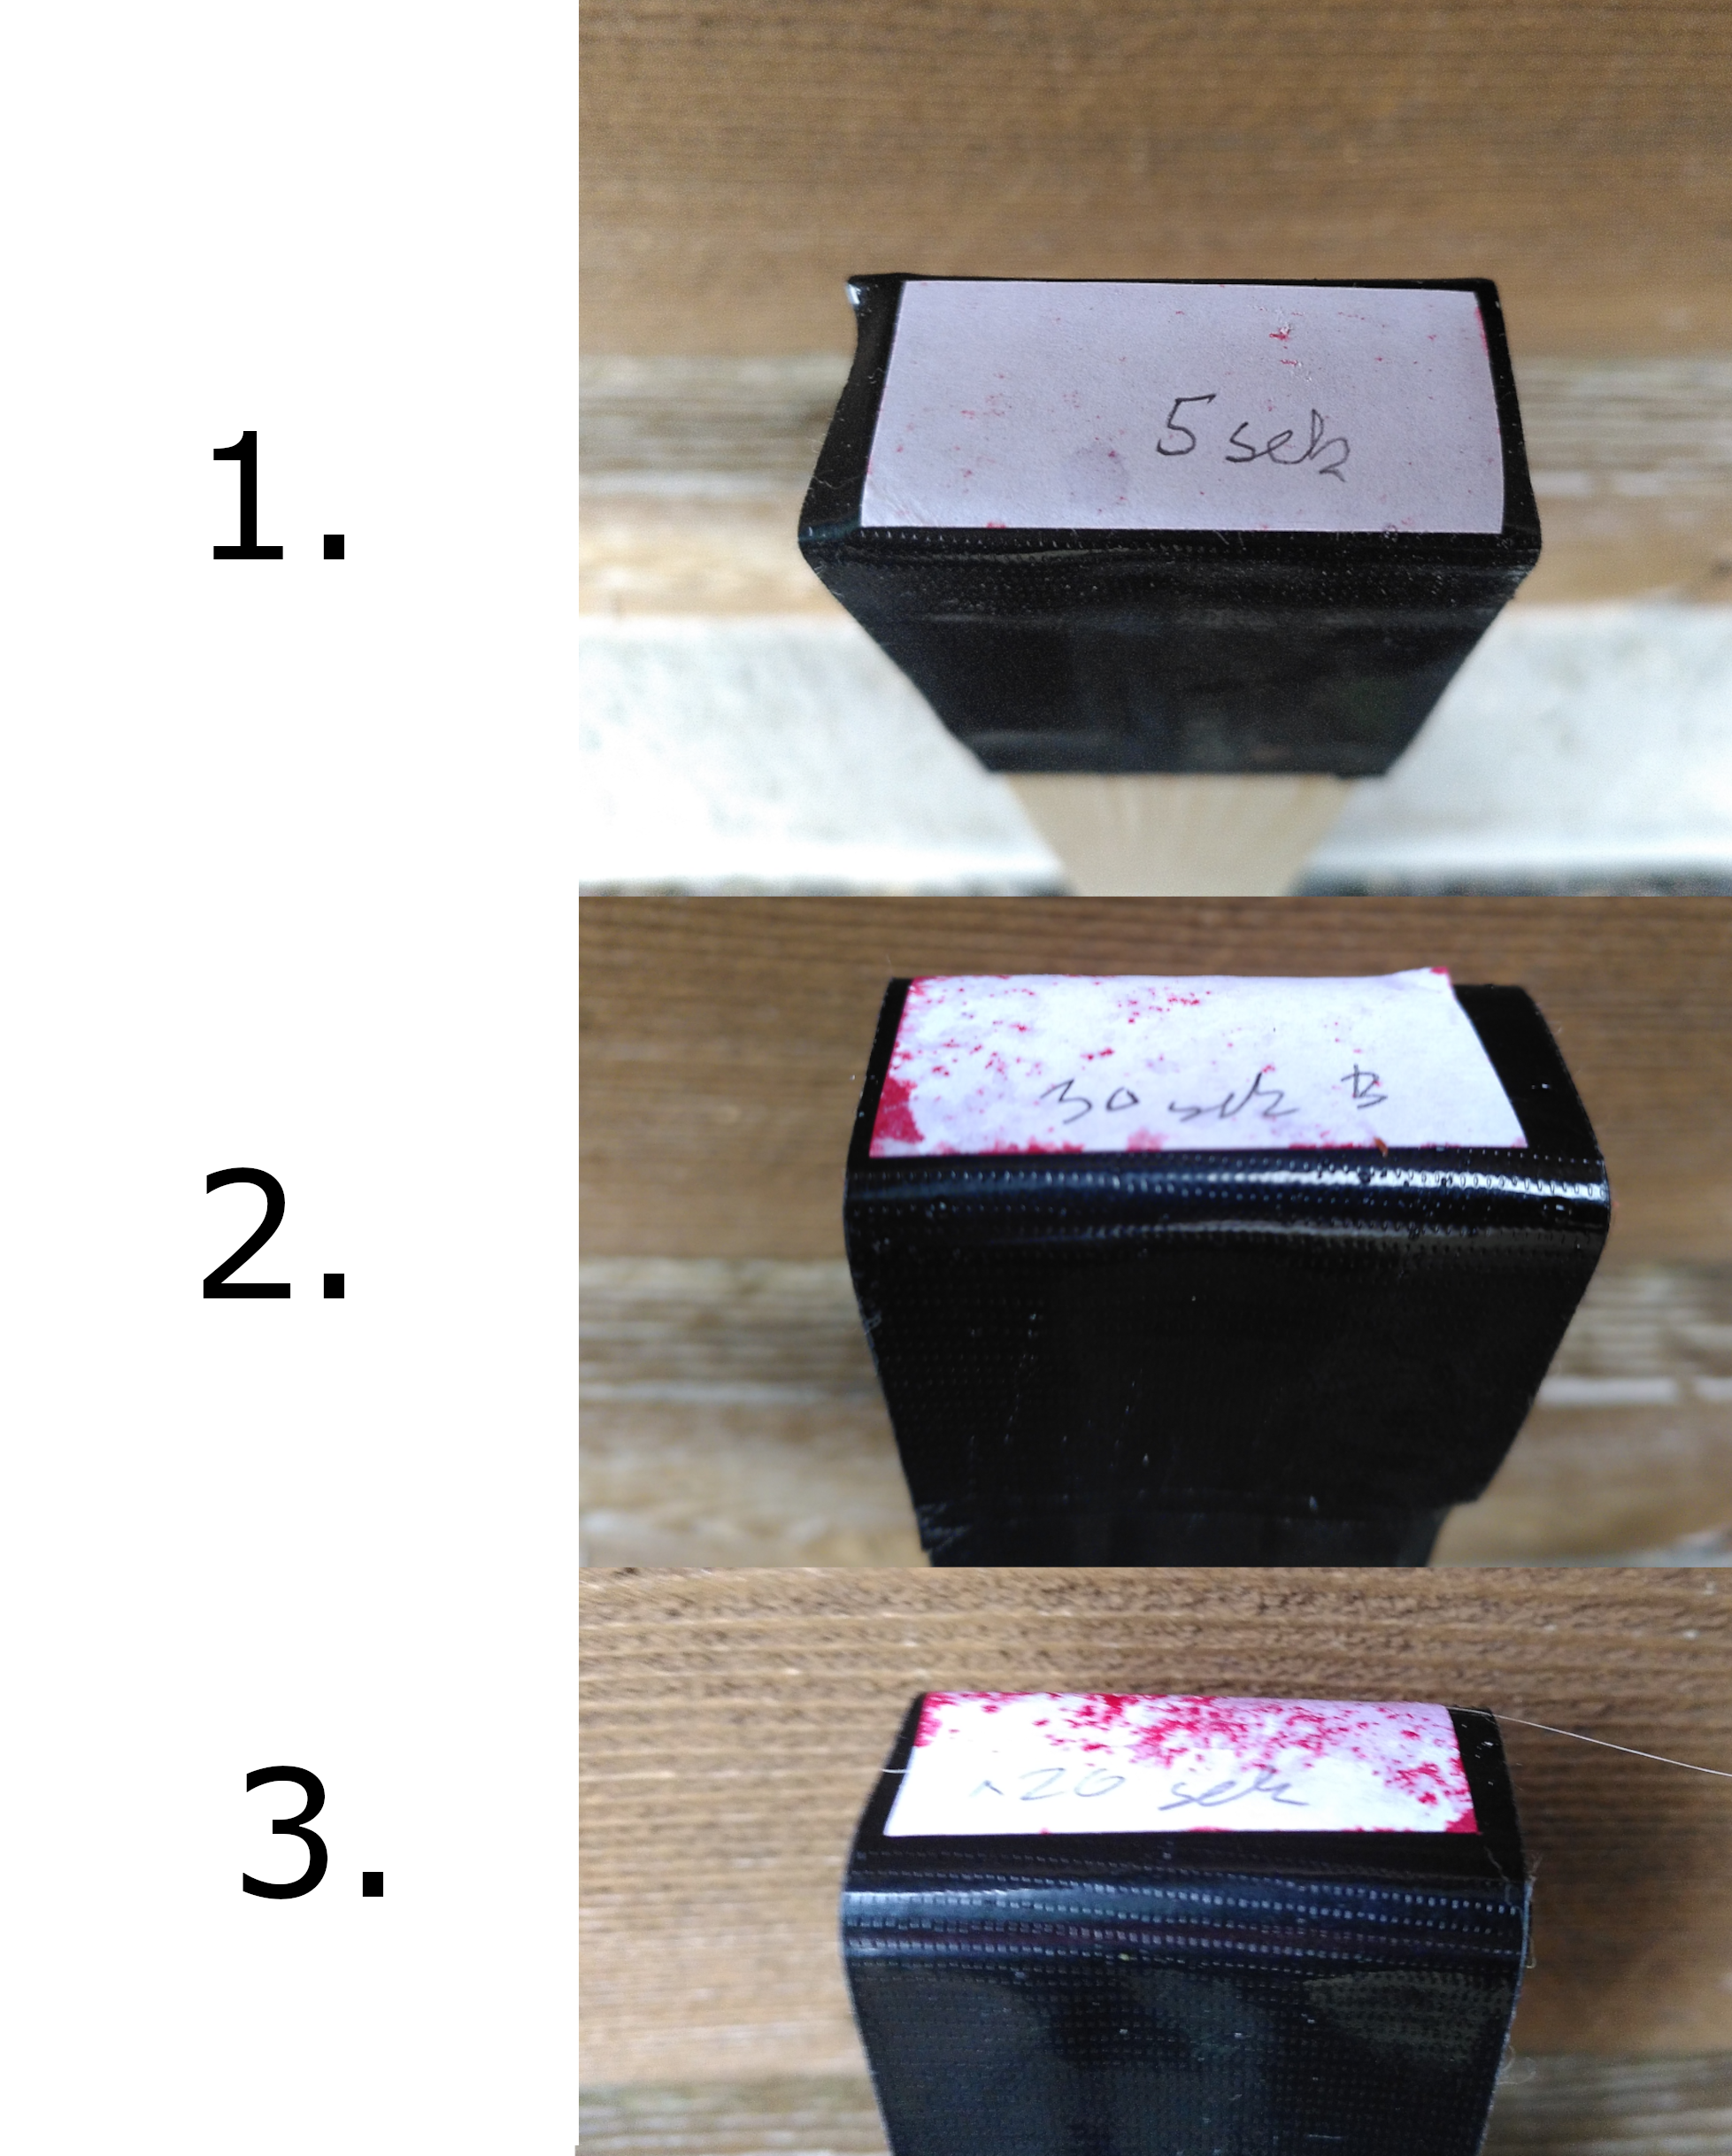
\includegraphics[width=0.8\textwidth]{Bilder/ZeitAbha.png}
    \caption{Drei Tapes gemessen bei nassem Schnee, da es geregnet hat: 1. 5 Sekunden Anpresszeit, 2. 30 Sekunden Anpresszeit, 3. 120 Sekunden Anpresszeit} 
    \label{fig:ZeitDruck}
\end{figure}

\newpage
\textbf{Zweiter Feldversuch}
\label{zweitFeldVer}
Ziel des zweiten Versuchs \ref{fig:DavosMessung} war es, den Ablauf der Tape-Messung bei verschiedenen LWC-Werten zu testen. Dazu wurde Schnee einmal mit Wasser übergossen und einmal mit Kältespray eingefroren. Die Ergebnisse sind in \ref{fig:DavosMessung} dargestellt. Die Wärmebildaufnahme \ref{fig:KaltSchnee} zeigte, dass der Schnee nur lokale Terperaturänderung macht, da Schnee gut isoliert. 

\begin{figure}[H]
    \centering
    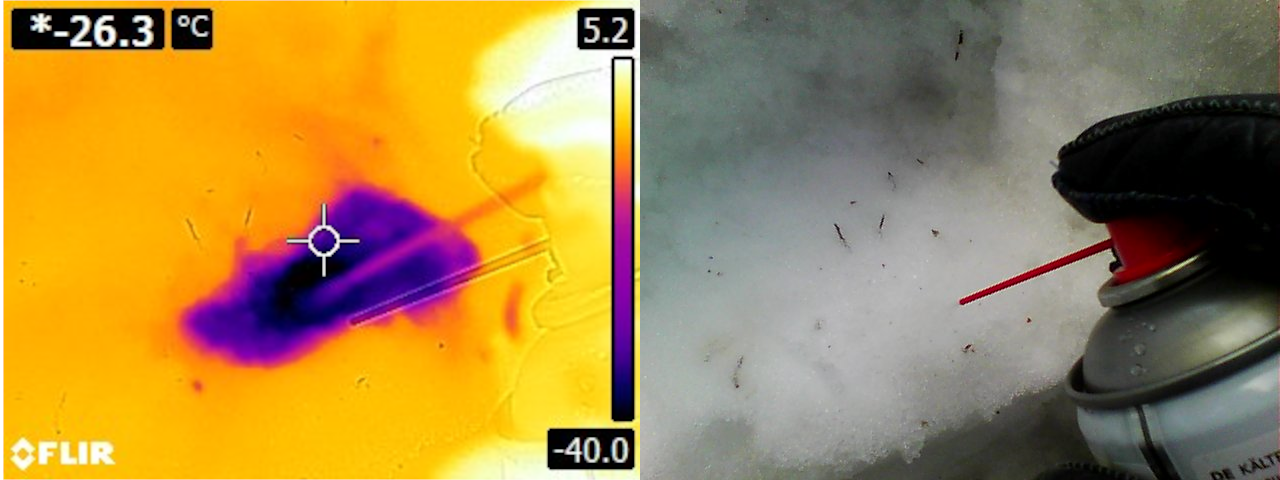
\includegraphics[width=0.8\textwidth]{Bilder/KalterSchnee.png}
    \caption{Wärmebildaufnahme der gekühlten Schneestelle, welche zur Simulation eines niedrigen LWC verwendet wurde.} 
    \label{fig:KaltSchnee}
\end{figure}



\begin{figure}[H]
    \centering
    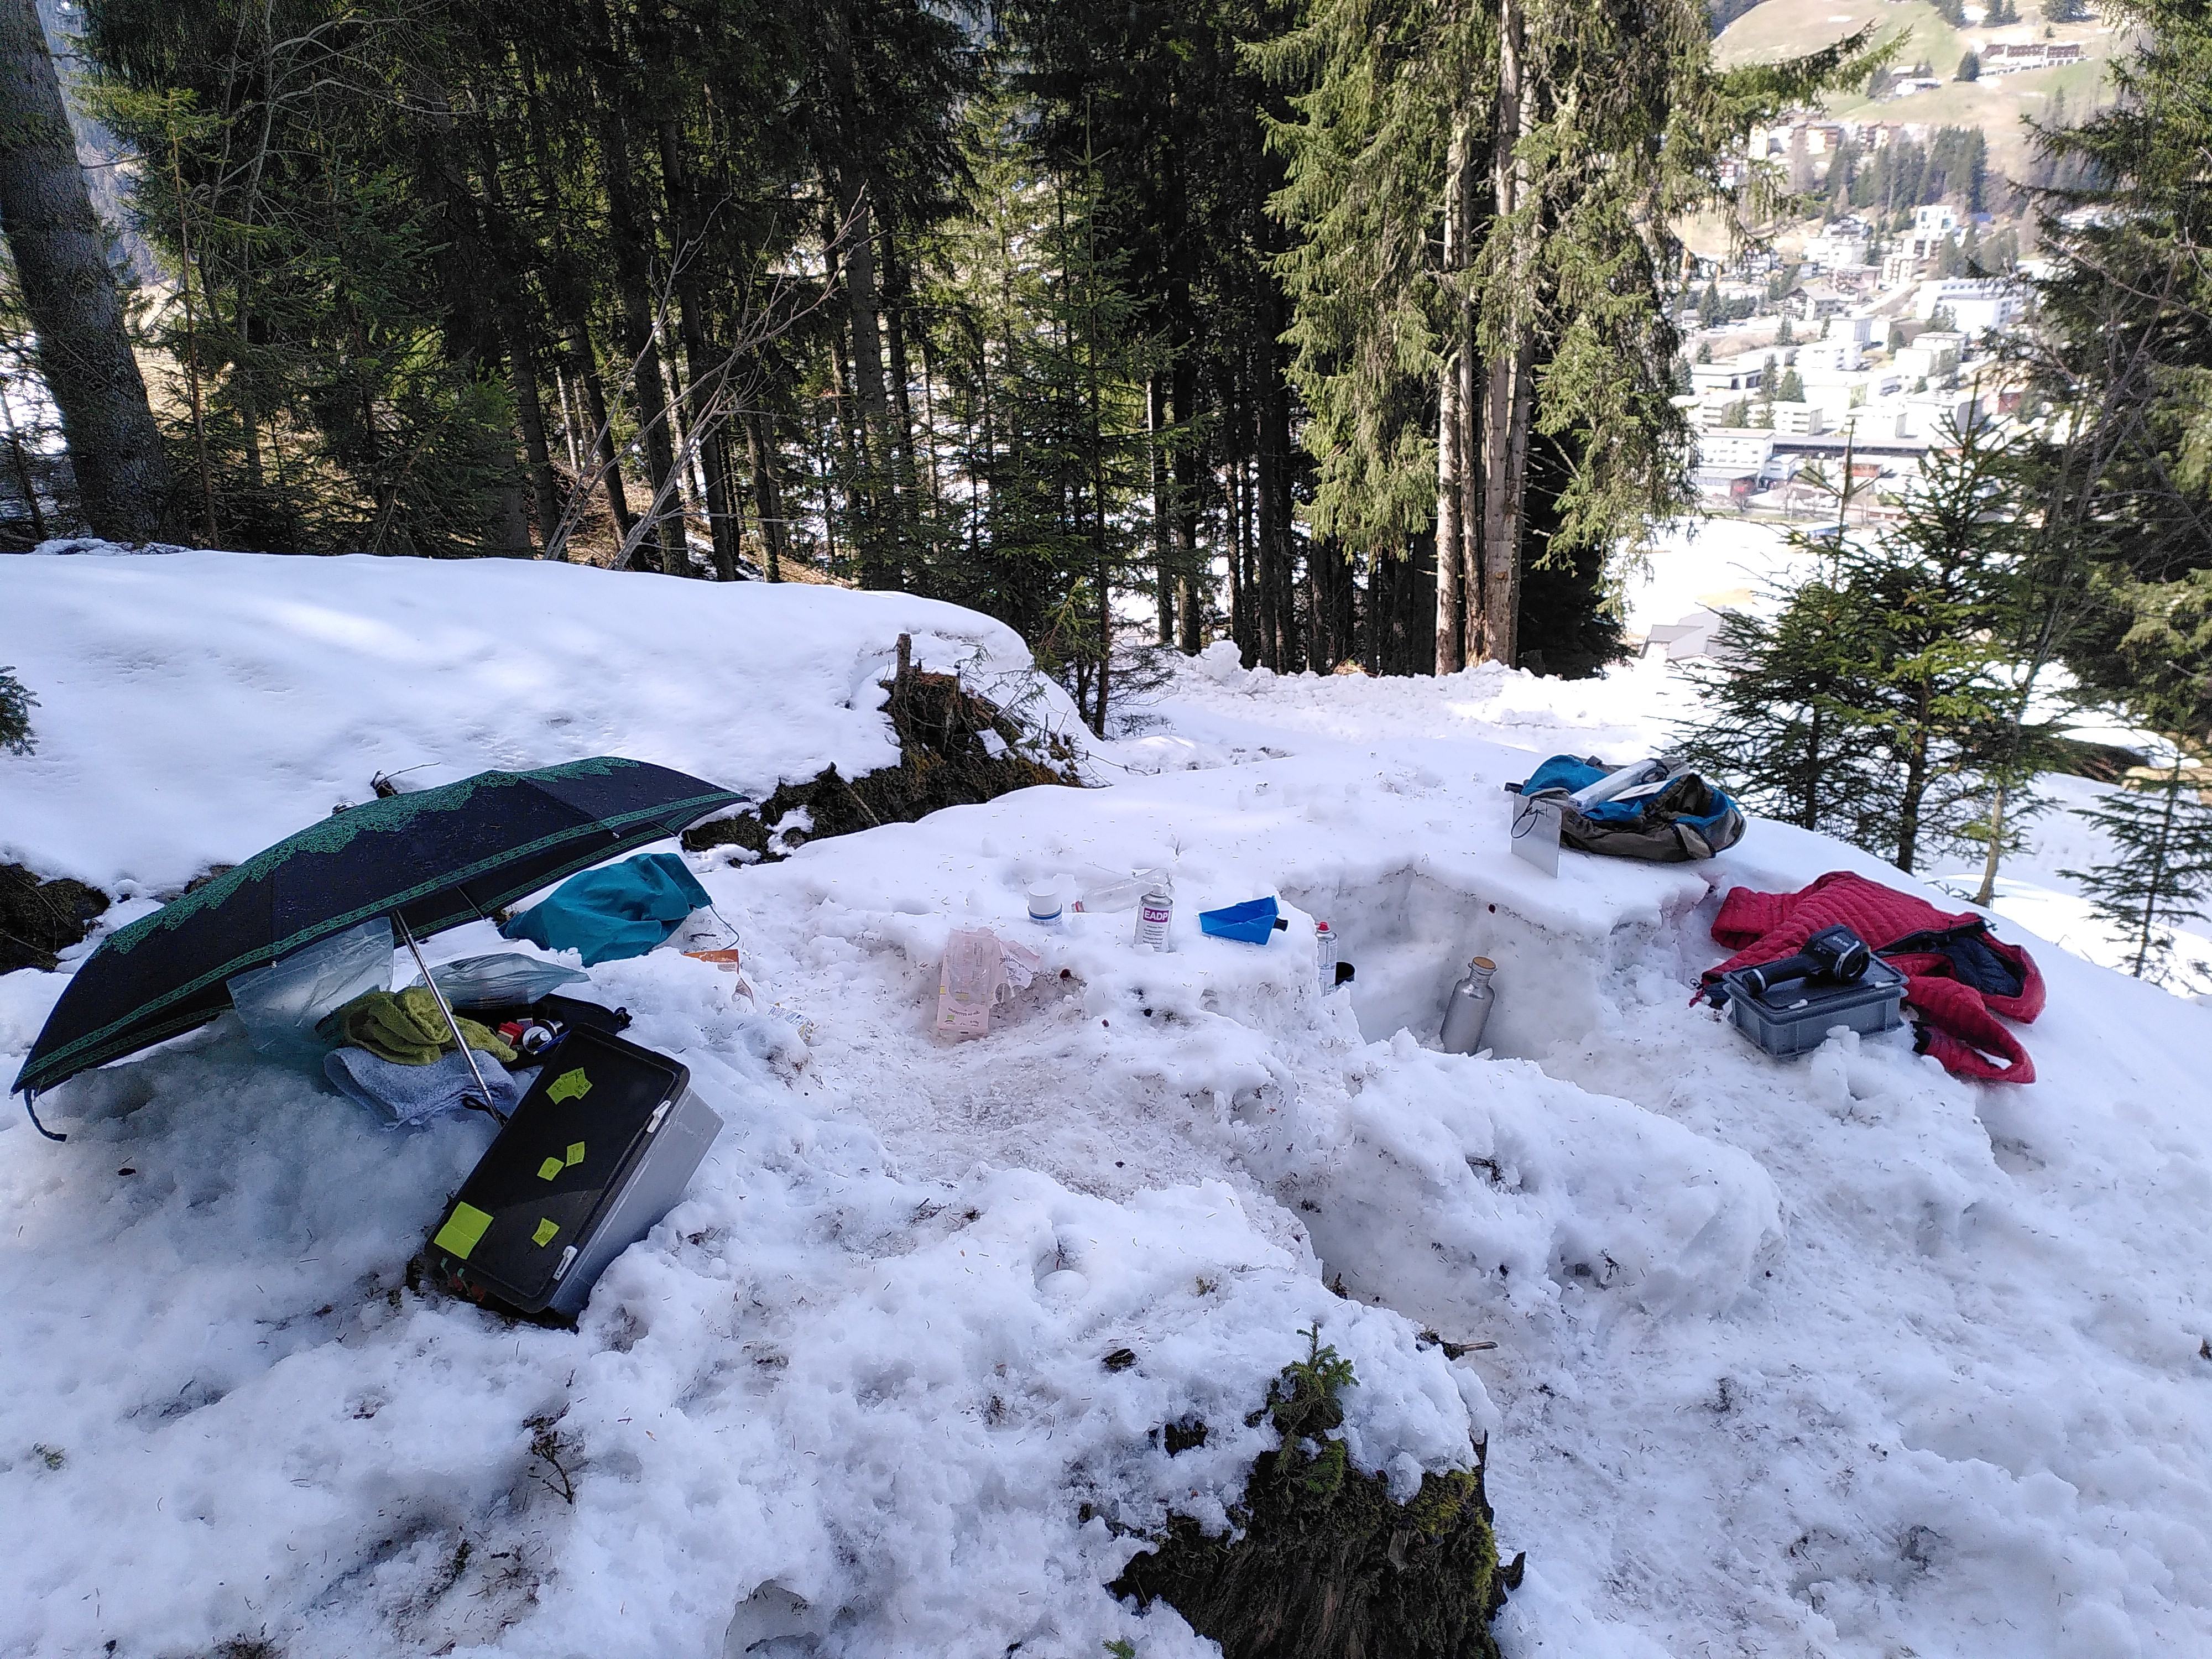
\includegraphics[width=0.8\textwidth]{Bilder/IMG_20240411_124421.jpg}
    \caption{Messstandort in Davos, unter dem Regenschirm ist das Tape gelagert, um es vor direkter Sonneneinstrahlung und Wasser Tropfen zu schützen.} 
    \label{fig:DavosMessung}
\end{figure}

\begin{figure}[H]
    \centering
    \includegraphics[width=0.8\textwidth]{Bilder/UnterschiedlicheLWC.png}
    \caption{Tapes aus dem ersten Feldversuch: 1. Unveränderter Schnee, 2. Gekühlter Schnee (siehe Abb. \ref{fig:KaltSchnee}),  3. Mit flüssigem Wasser übergossener Schnee.} 
    \label{fig:DavosMessung}
\end{figure}


%\caption{Ein bild von 'normalem' schnee}
\newpage

\textbf{dritter Feldversuch}
\label{drittFeldVer}

\begin{figure}[H]
    \centering
    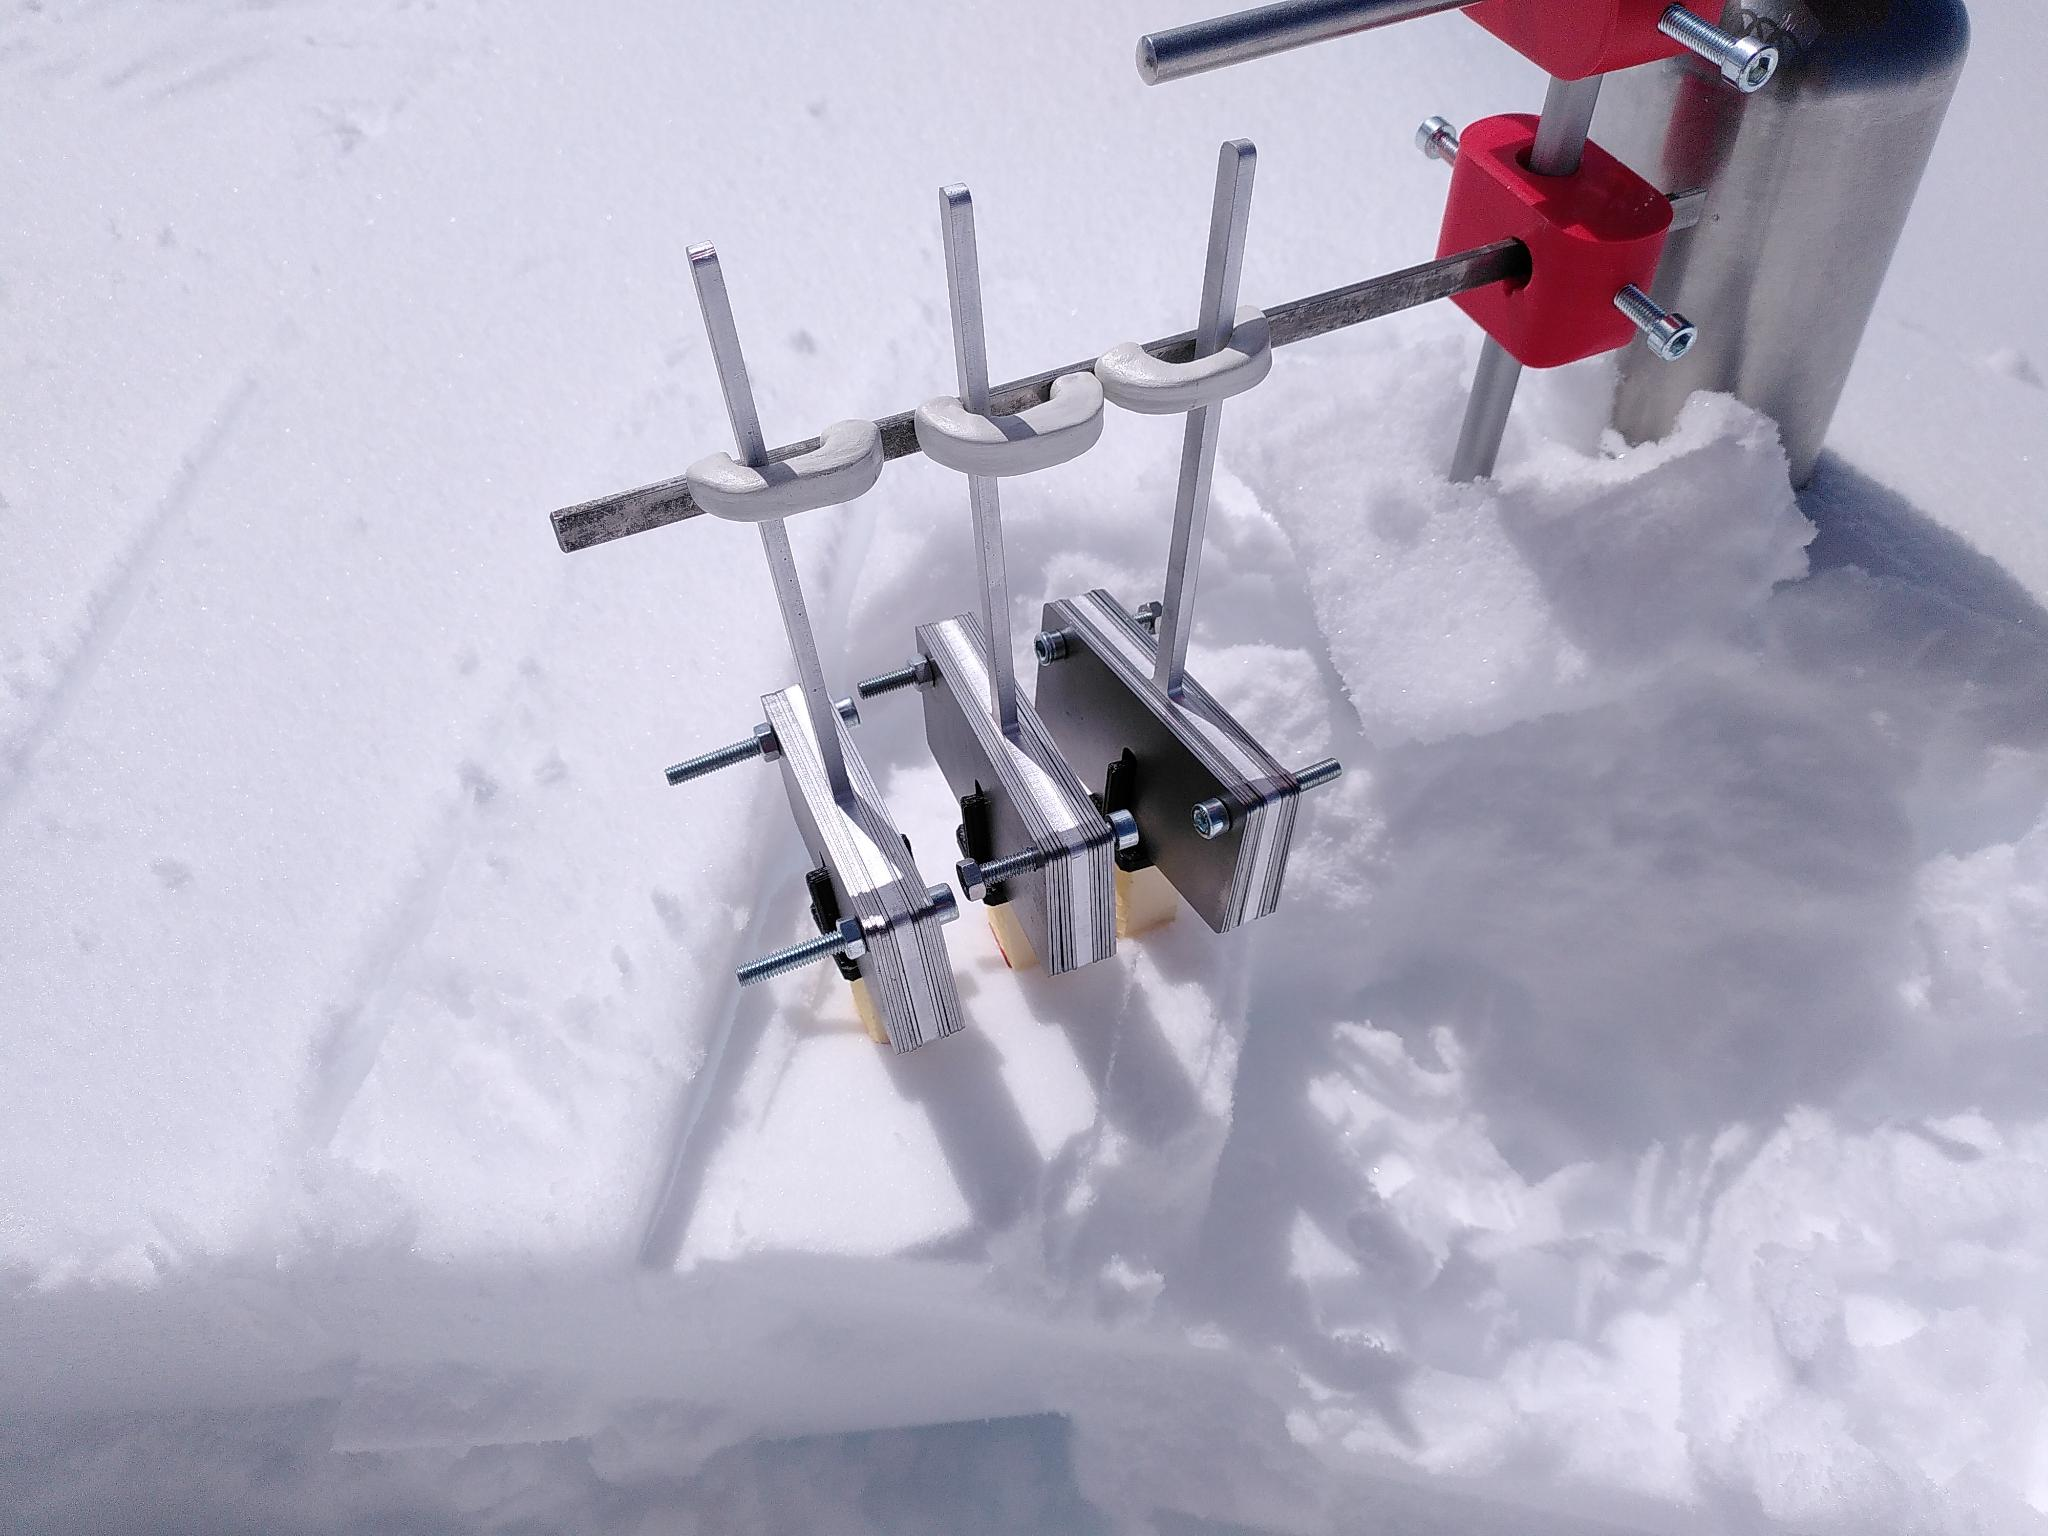
\includegraphics[width=0.8\textwidth]{Bilder/aufbauTitlis.jpeg}
    \caption{Messaufbau von drei Tapes auf unverändertem Schnee} 
    \label{fig:aufbauTitlis}
\end{figure}
Im dritten Versuch \ref{fig:aufbauTitlis} wurde ein neues Design mit variablem Anpressdruck getestet. Es zeigte sich, dass die Varianz am geringsten war, wenn das Gewicht 80\% der maximalen Tragkraft des Schnees betrug. In \ref{fig:12Palt} ist das Ergebnis zu sehen.

\begin{figure}[H]
    \centering
    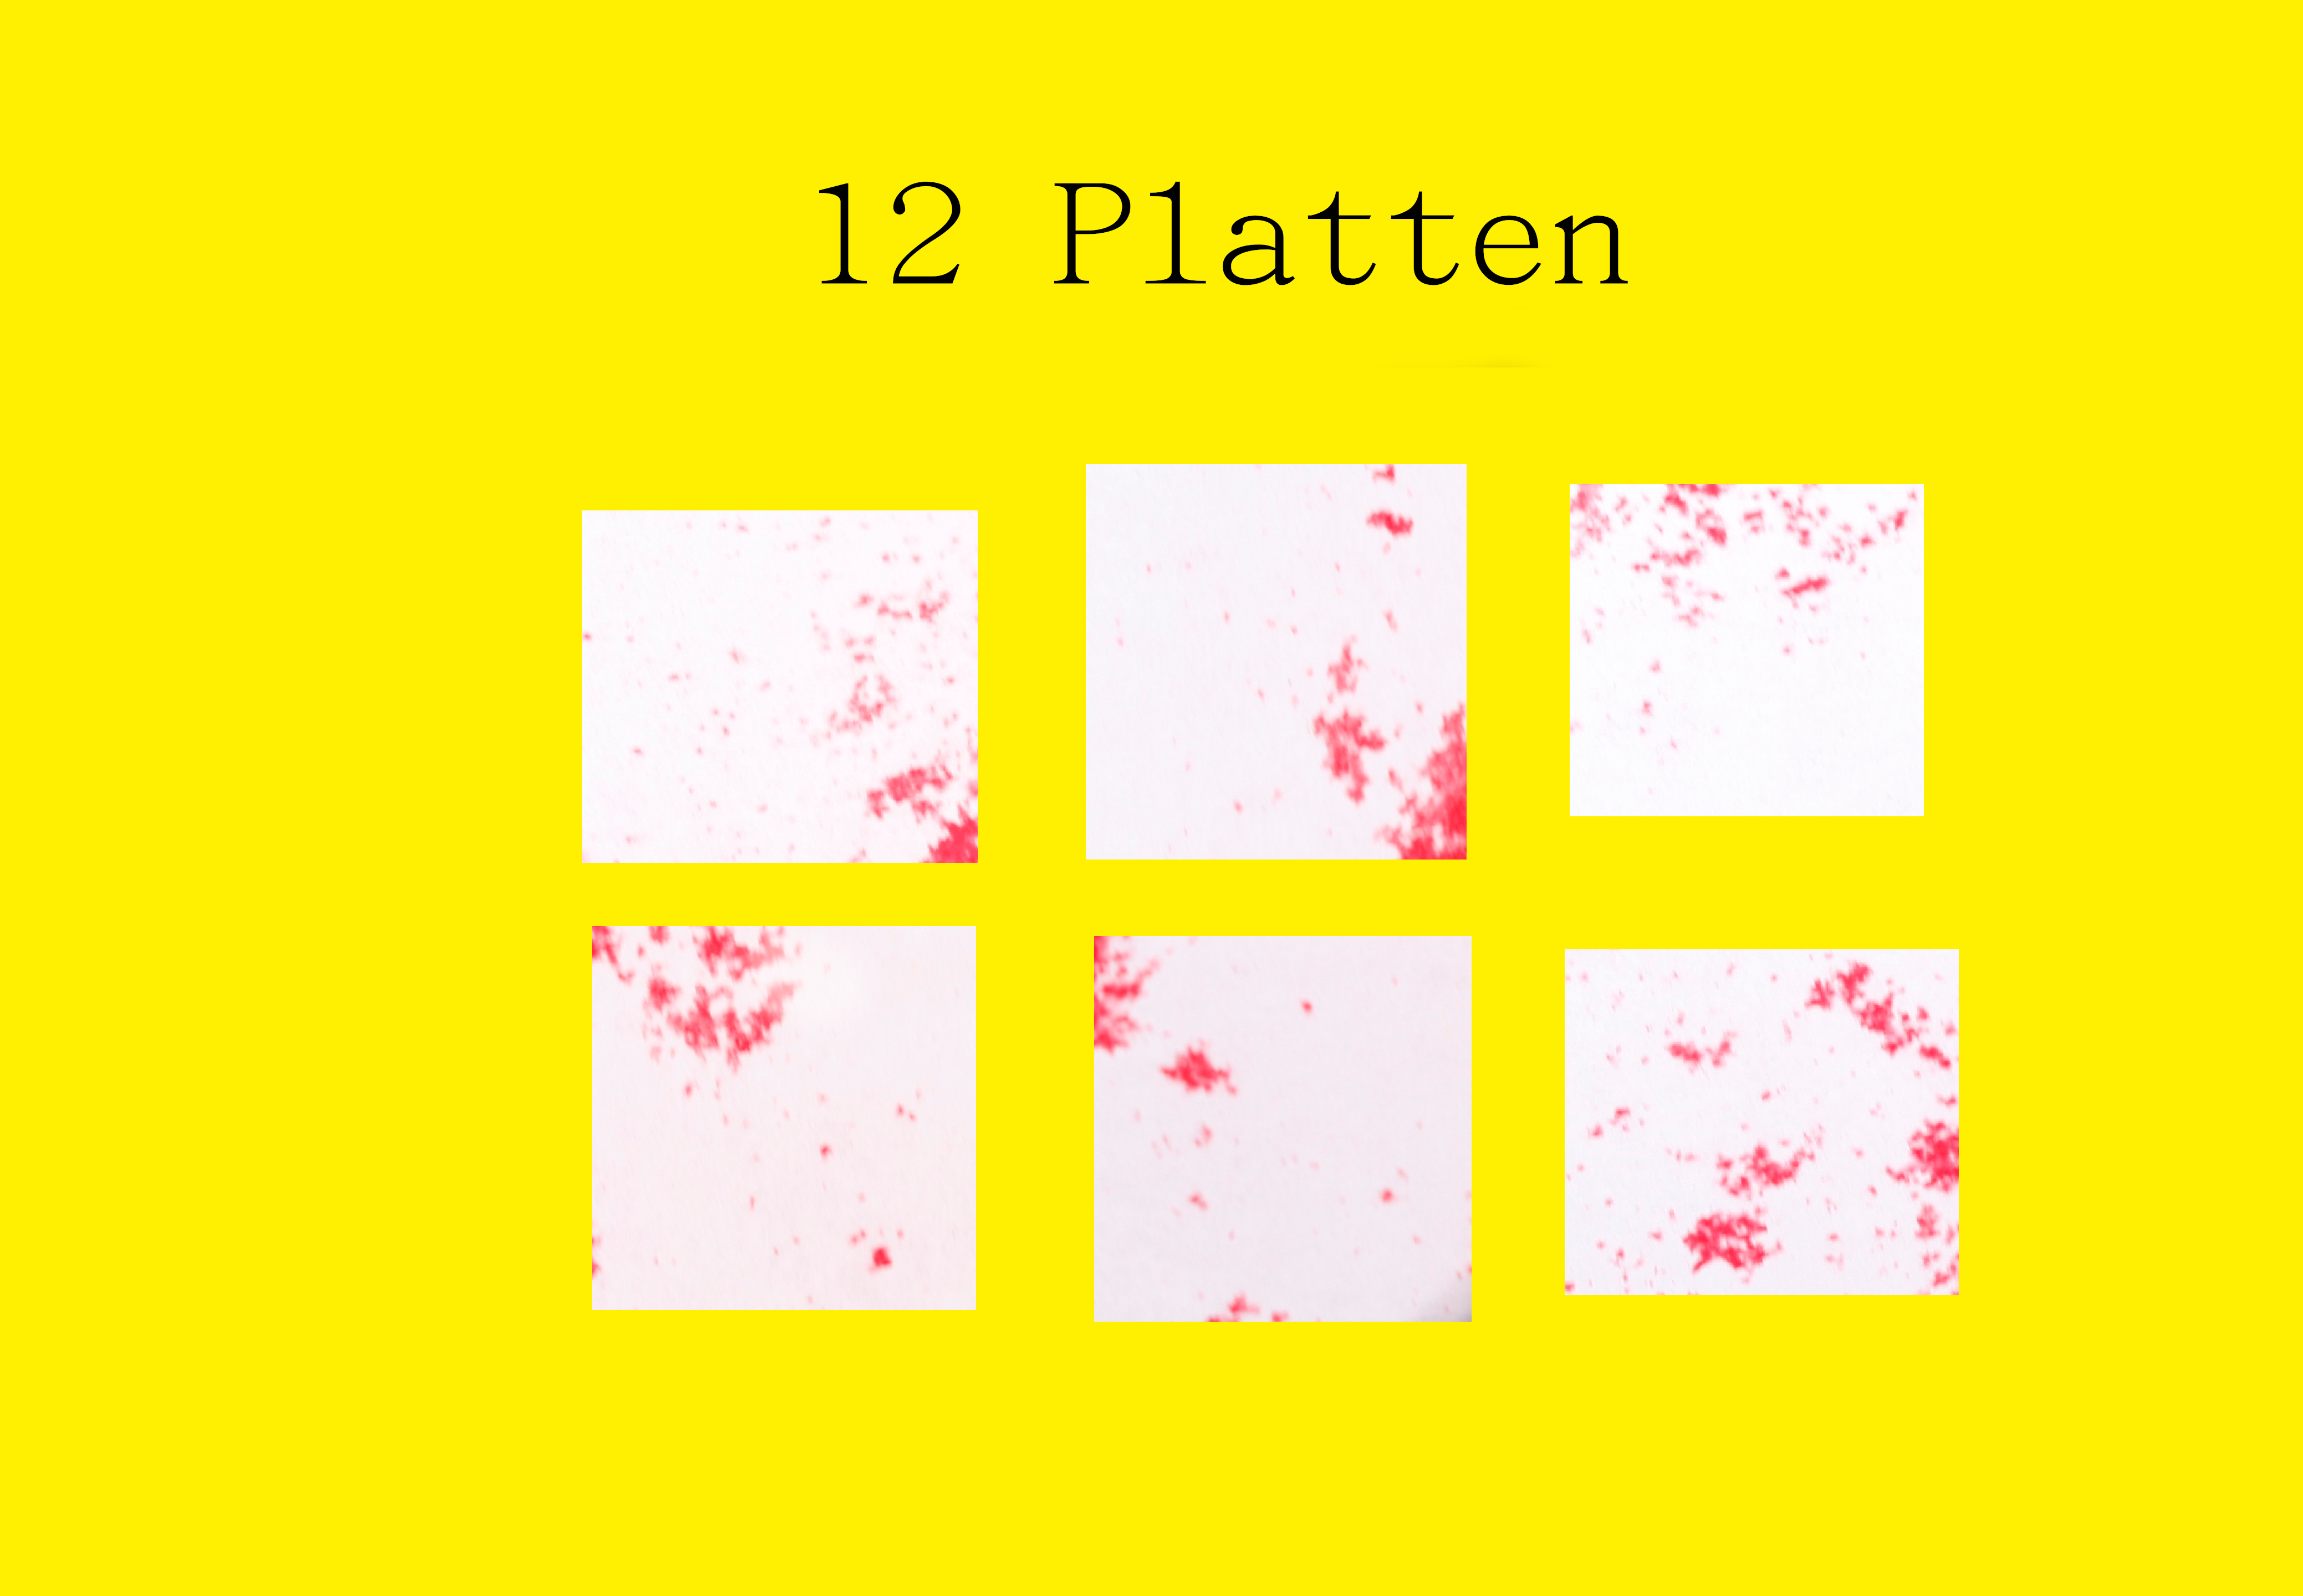
\includegraphics[width=0.8\textwidth]{Bilder/12Platten.png}
    \caption{Messung von sechs Tapes mit  zwölf Stahlplatten und einem Gesamtgewicht von 514 g auf unverändertem Schnee, um die Varianz der Messergebnisse zu bestimmen.} 
    \label{fig:12Palt}
\end{figure}

\newpage
Es wurde auch untersucht, wie sich das Tape verhält, wenn derselbe Schnee mehrmals hintereinander getestet wird. Dabei zeigte sich, dass die Menge an Wasser, die benötigt wird, um das Tape zu befeuchten, während der 120 Sekunden Andruckzeit vom Schnee bereitgestellt werden kann. \ref{fig:aufbauTitlis}


\begin{figure}[H]
    \centering
    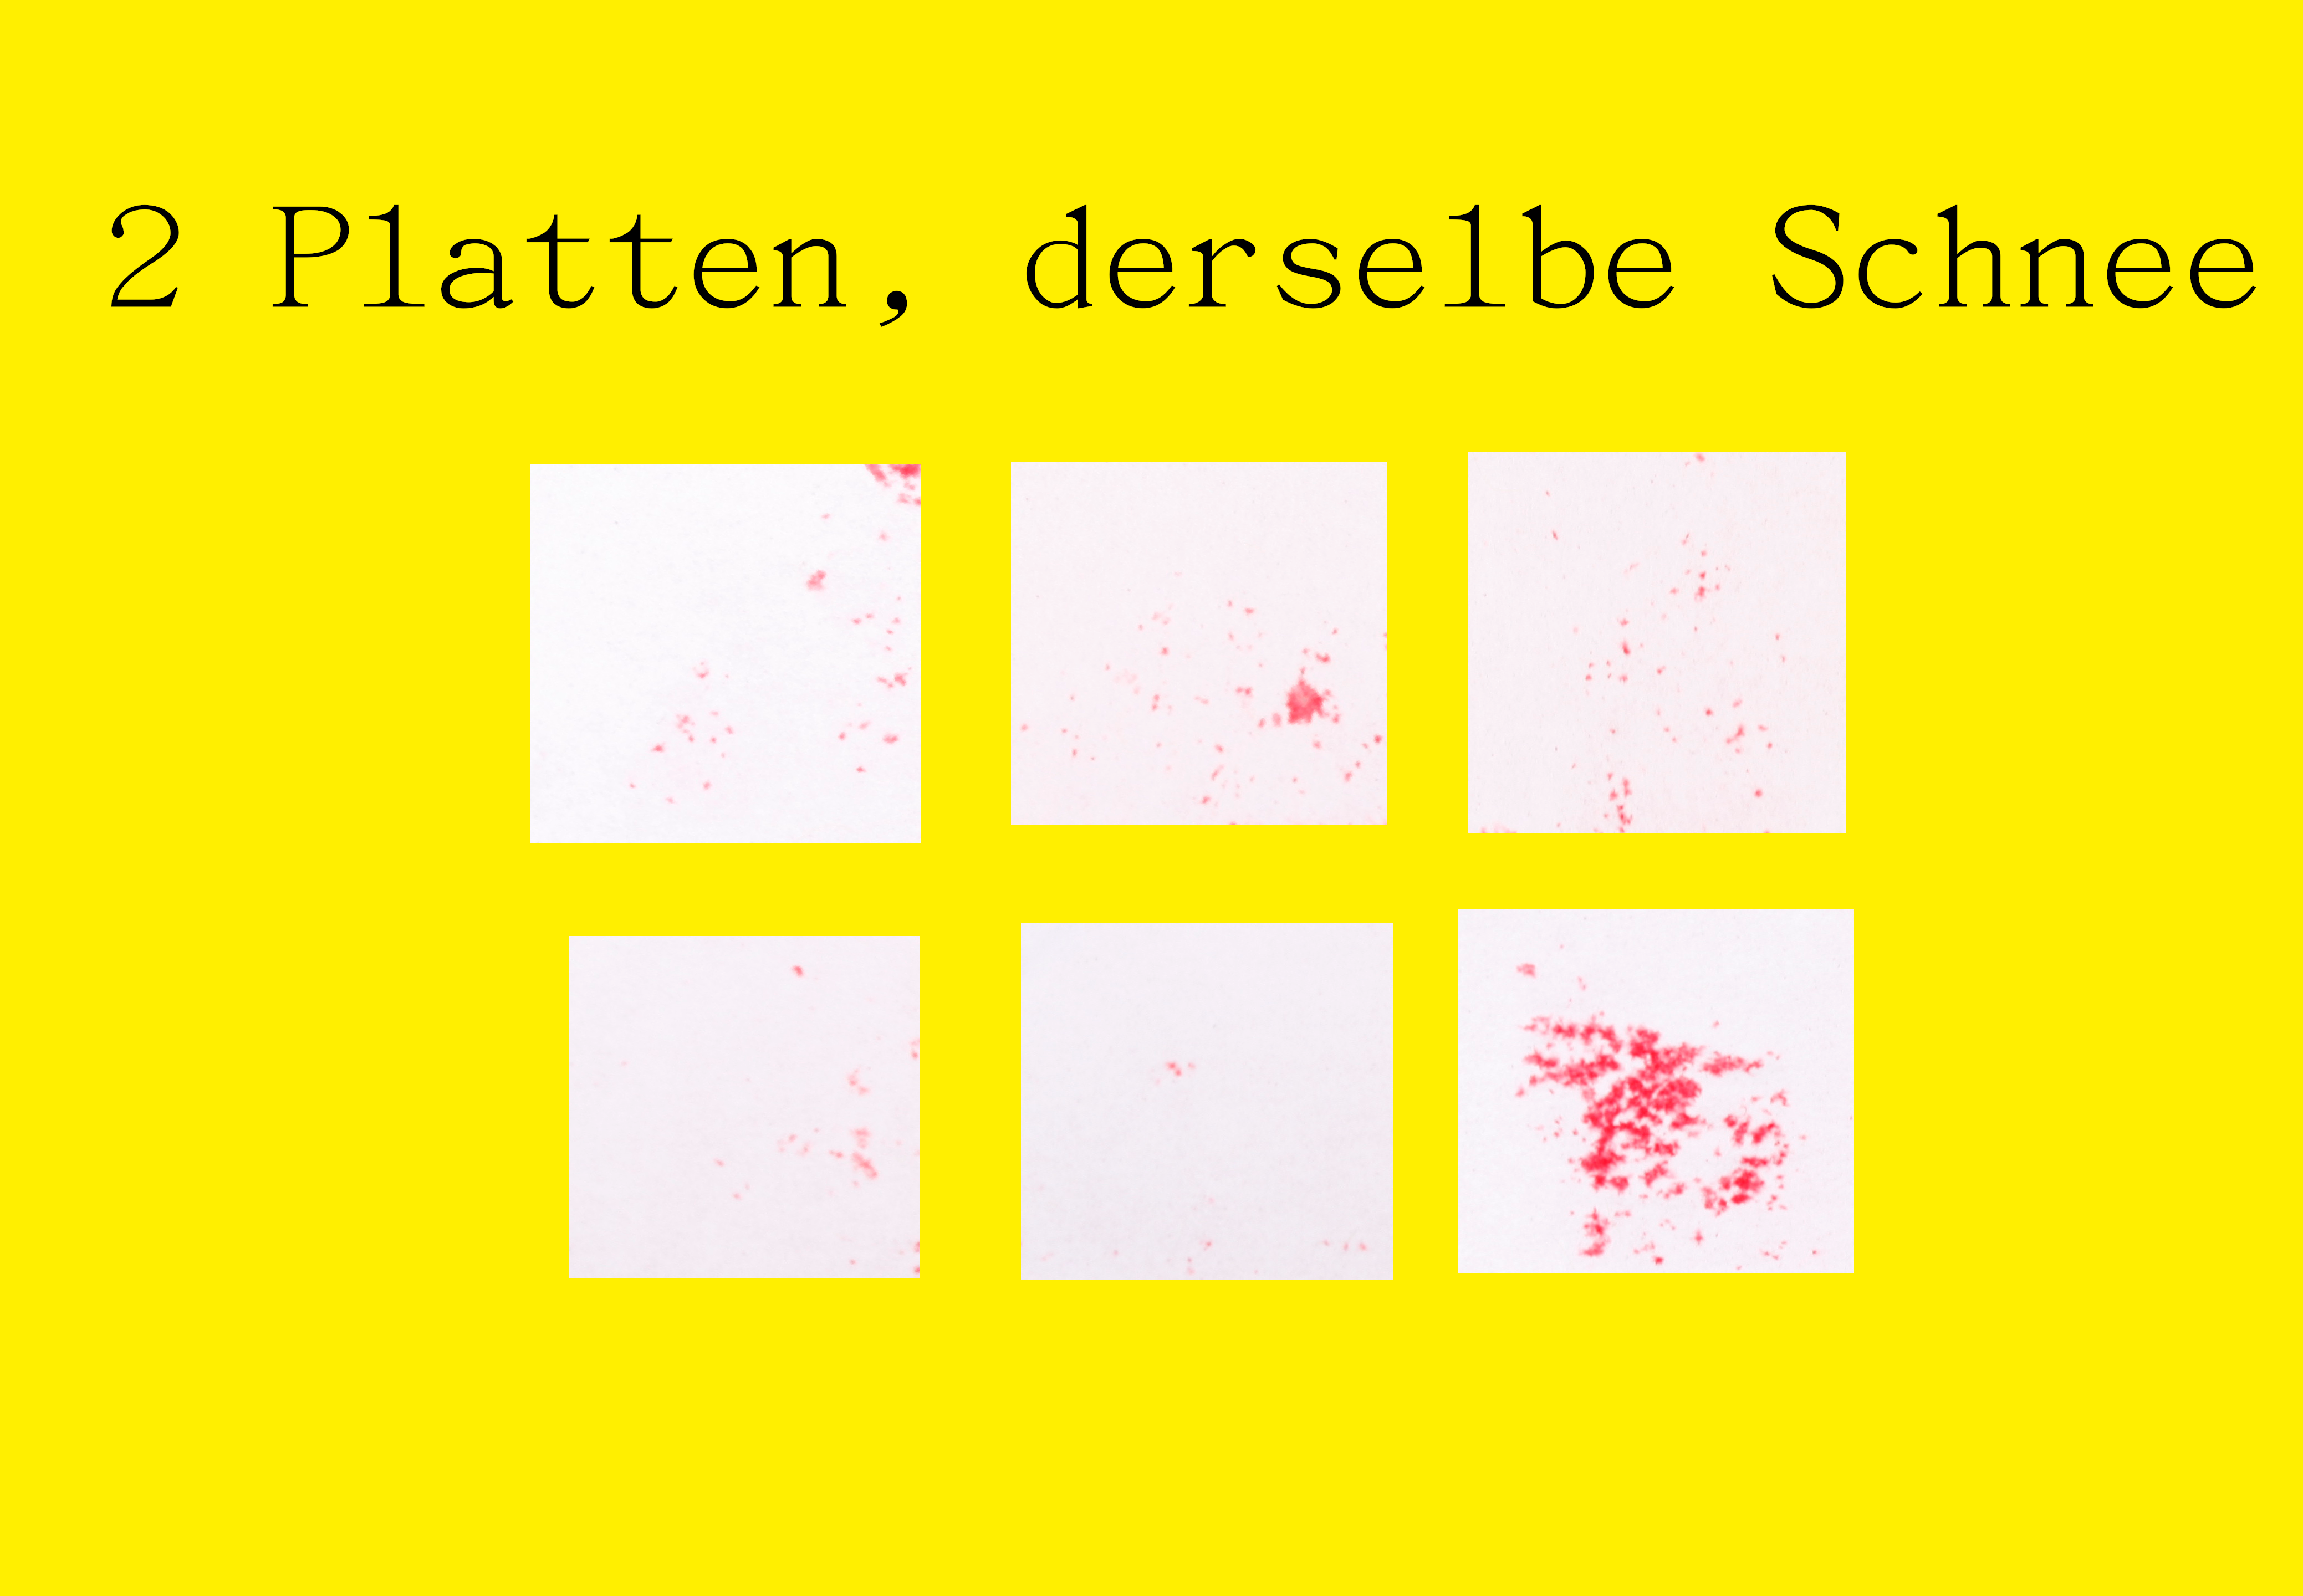
\includegraphics[width=0.8\textwidth]{Bilder/2PlattenSelberSchnee.png}
    \caption{Messung von sechs Tapes auf dem selben unverändertem Schnee, um die Einflüsse des Messen auf den Schnee zu erkennen.} 
    \label{fig:aufbauTitlis}
\end{figure}


\subsection{Vergleich der Ergebnisse mit Denothmeter}
Das Ziel ist es die Statistik Daten aus \ref{} zu benutzten um ein statischtisches Regressions maschien learn modell auf zu bauen. der Input sind dann parameter wie zum beistiel das RedVsWhite oder der RadiusAvg. der output ist der LWCTape. um das modell zu trainiern wird der LWCDenoth benutzt.

dass heisst im besten fall kann das Tape die gleichen Werte wie das Denothmeter produzieren. aber mit dieser technik ist es nicht möglich eine qualitativ bessere über schnee und Gleitschneelawinen zu machen als das denothmeter.

Um ein modell zu trainiern das den Denothmeter gut abbieldet, muss das modell mit möglichst vielen schneetypen und entsprechenden LWCDenoth trainiert werden.

mein bauchgefühl sagt, dass für ein rubustes modell 100 LWCDenoth gut wären. Das gute an ML ist, dass die genauigkeit der modelle weitgehen linear mit der  anzahl traingsdaten steigt.

\caption{grafik aus der Vorlesung Deep Learning, Hannes Badertsch}

In den frühen phasen diesr BA wird nur das Konzept eingeführt und dan das eigene biologische neuronale Netztwerk im Hirn benutzt um die Bilder/Statisik mit den LWCDenoth zu korrelieren.

das ist die Userstory von XX aus \ref{}


um eine aussage über gleitschneelawinen zu machen die besser ist als die des Denothmeters, müssen die entsprechenden Daten gesammelt werden. dass heisst es braucht eine messkampanie die  kritische Hänge überwacht und dann kann das klassifikations modell trainiert werden, dass eine Serie von Tape Roh daten betrachtet und als output hat: Jetzt wird eine Gleitschneelawine statfinden.

das ist die Userstory von x aus \ref{}


\subsection{Verbesserungsmöglichkeiten des Funktionsmusters}
die geometrie des tapes ist

zwischen dem tape und dem gewicht kann ein flexibler schaumstoff eingesetzt werden, so konnte sich das tape an die unregemasigkeit des schnees besser anpassen.

das tape kann mit einer membran an der schnee gedruckt werden. so kann auf die kraft praktischer kontroliert werden. schwerkraft ist nicht praktisch um eine vollautomatisches produkt zu entwicklen.

die geometrie des harten xps schaums konnte durch eine Kegel ersetzt werden, so kann eine andere andruckkraft erreicht werden.


\newpage
\section{Ausblick}
lovly


\subsection{Presönliche Erfahrunng}


Ich hatte Freude mich in das mir unbekannte Thema des Schnees einzuarbeiten. Die Arbeit hat mir einen kleinen Einblick in den Schnee gegeben, das Thema des Schnees wird für die Schweiz in den kommenden Jahren mit dem Klimawandel an Bedeutung gewinnen.

Die agile Hardware Development Methode liegt mir und es hat Freude bereitet 5 Iterationen des Produktes in der Hand zu haben und zu testen.


\subsection{Fazit}
Die Erkenntnisse und Ergebnisse dieser Arbeit bieten eine solide Grundlage für zukünftige Entwicklungen und Forschungen im Bereich der Schneemessung. dass das Konzept vielversprechend ist und weiterhin potenzielle Verbesserungen und Anpassungen ermöglicht.
Entwicklung eines Messablauf mit dem Water indicator tape

verschiedene 5 ausprobierte, 3 erflogreich, 1 weiter entwickelt

nicht nur lwc sonder auch hoffnung auf geometrie des schnees

halbe seite


\subsection{Ausblick}
Der weitere Verlauf der Forschung sollte darauf abzielen, die Präzision und Genauigkeit der Schneemessung zu erhöhen sowie die Anwendbarkeit des Systems in verschiedenen Umgebungen zu testen. Dabei sollten auch mögliche Verbesserungen im Hinblick auf die Automatisierung der Messungen und die Reduzierung des Arbeitsaufwands berücksichtigt werden.

Eine entscheidende Fragestellung besteht darin, die beobachtete Varianz in den Messungen zu verstehen. Es ist wichtig zu klären, ob diese Varianz auf Unterschiede im Liquid Water Content (LWC) des Schnees zurückzuführen ist oder ob sie einen Effekt der Messung selbst darstellt. Um eine statistisch fundierte Aussage treffen zu können, sollten über 30 Messungen von vergleichbaren Schneeproben durchgeführt werden.

Um die statistische Basis der Datenbank zu verbessern, sollten über 1000 Messungen mit dem Tape und etablierten LWC-Messwerten durchgeführt werden. Dadurch können die Daten analysiert, validiert und das Messsystem weiterentwickelt werden.


\newpage
% Literaturverzeichnis
%\bibliography{mybibliography}
\section{Literaturverzeichnis}



\begin{thebibliography}{9}

\bibitem{hypecycle} \url{https://www.gartner.com/en/articles/what-s-new-in-the-2023-gartner-hype-cycle-for-emerging-technologies}{Gartner Hype Cycle for Emerging Technologies 2023}, abgerufen am 19.12.2023

\bibitem{TempLink}  \url{https://www.schweizer-fn.de/stoff/waermedehnung/waermedehnung.php}{Temperature Expansion Tutorial}, abgerufen am 19.12.2023

\bibitem{SchwindungLit}   Christian Bonten. \textit{Kunststofftechnik: Einführung und Grundlagen}. Carl Hanser Verlag GmbH \& Co. KG, München, 3. aktualisierte edition, 2020.

\bibitem{VorlesungSML} Badertscher, H.: Vorlesung Statistical Machine Learning 2023
\bibitem{VorlesungKT} Ehrig, F. und Andere: Vorlesung Konstruieren mit Kunststoffen 2023
\bibitem{VorlesungDB} Schwab, J.: Vorlesung Datenbanksysteme 1 2023
\bibitem{VorlesungWah} Tietje, O.:Vorlesung Wahrscheinlichkeit und Messdaten 2022
\bibitem{VorlesungPyt} Malacarne S.:Vorlesung Python 2023
\bibitem{MAJaps} Hollender, J.: Vorhersage der Qualitätsmerkmale von Spritzgussbauteilen nach 24h anhand von Korrelationsmodellen 2021, unveröffentlichte Masterarbeit an der OST, Betreuer: Frank Ehrig
\bibitem{MAGew} Stocker, C.: Datengetriebene Prädiktion des Bauteilgewichts von Spritzgiessbauteilen 20221, unveröffentlichte Semesterarbeit an der OST, Betreuer: Frank Ehrig
\bibitem{SwissAI} \url{https://www.swissinfo.ch/eng/business/swiss-initiative-aims-for-global-leadership-in-ai/49029736}, abgerufen am 19.12.2023
\bibitem{VorlesungMess} Šeatović, D.: Vorlesung Messtechnik 2022
\bibitem{ChatGPT} ChatGPT
\bibitem{GPT4All} GPT4All mit Mistral OpenOrca LLM
\bibitem{WH} \url{https://www.wh.group/en/services/ruby/}
\bibitem{NewsP} \url{https://www.plasticstoday.com/injection-molding/how-artificial-intelligence-is-transforming-injection-molding}
\bibitem{NatureP} \url{https://www.nature.com/articles/s41598-023-48679-0}
\bibitem{ieeeP} \url{https://ieeexplore.ieee.org/document/8369500}
\bibitem{katulu} \url{https://katulu.io/en/solutions/briefs/ai-based-injection-molding/}

\end{thebibliography}



\newpage
\section{Erklärung zur Urheberschaft}


Ich erkläre hiermit, dass ich die vorliegende Arbeit ohne Hilfe Dritter angefertigt habe. Ich habe nur die Hilfsmittel benutzt, die ich angegeben habe. Gedanken, die ich aus fremden Quellen direkt oder indirekt übernommen habe, sind kenntlich gemacht. Die Arbeit wurde bisher keiner anderen Prüfungsbehörde vorgelegt und auch noch nicht veröffentlicht.

KI-Einsatz ohne Kennzeichnungspflicht

Ich bin mir bewusst, dass die Nutzung maschinell generierter Texte keine Garantie für die Qualität von Inhalten und Text gewährleistet. Ich versichere daher, dass ich den Text generierender KI-Tools lediglich als Hilfsmittel bedient habe und in der vorliegenden Arbeit meinen gestalterischen Einfluss überwiegt. Ich verantworte die Übernahme jeglicher von mir verwendeter maschinell generierter Textpassagen vollumfänglich selbst. Ich versichere, dass ich keine KI-Schreibwerkzeuge verwendet habe, deren Nutzung der Prüfer / die Prüferin explizit schriftlich ausgeschlossen hat.



Ort/Datum: Rapperswil, 2024 \\
Unterschrift:\\
Peter Kuhn


\newpage
\listoffigures


\listoftables % Tabellenverzeichnis erstellen
\newpage
\section{Digitaler Anhang}

\subsection*{Lebenslauf}
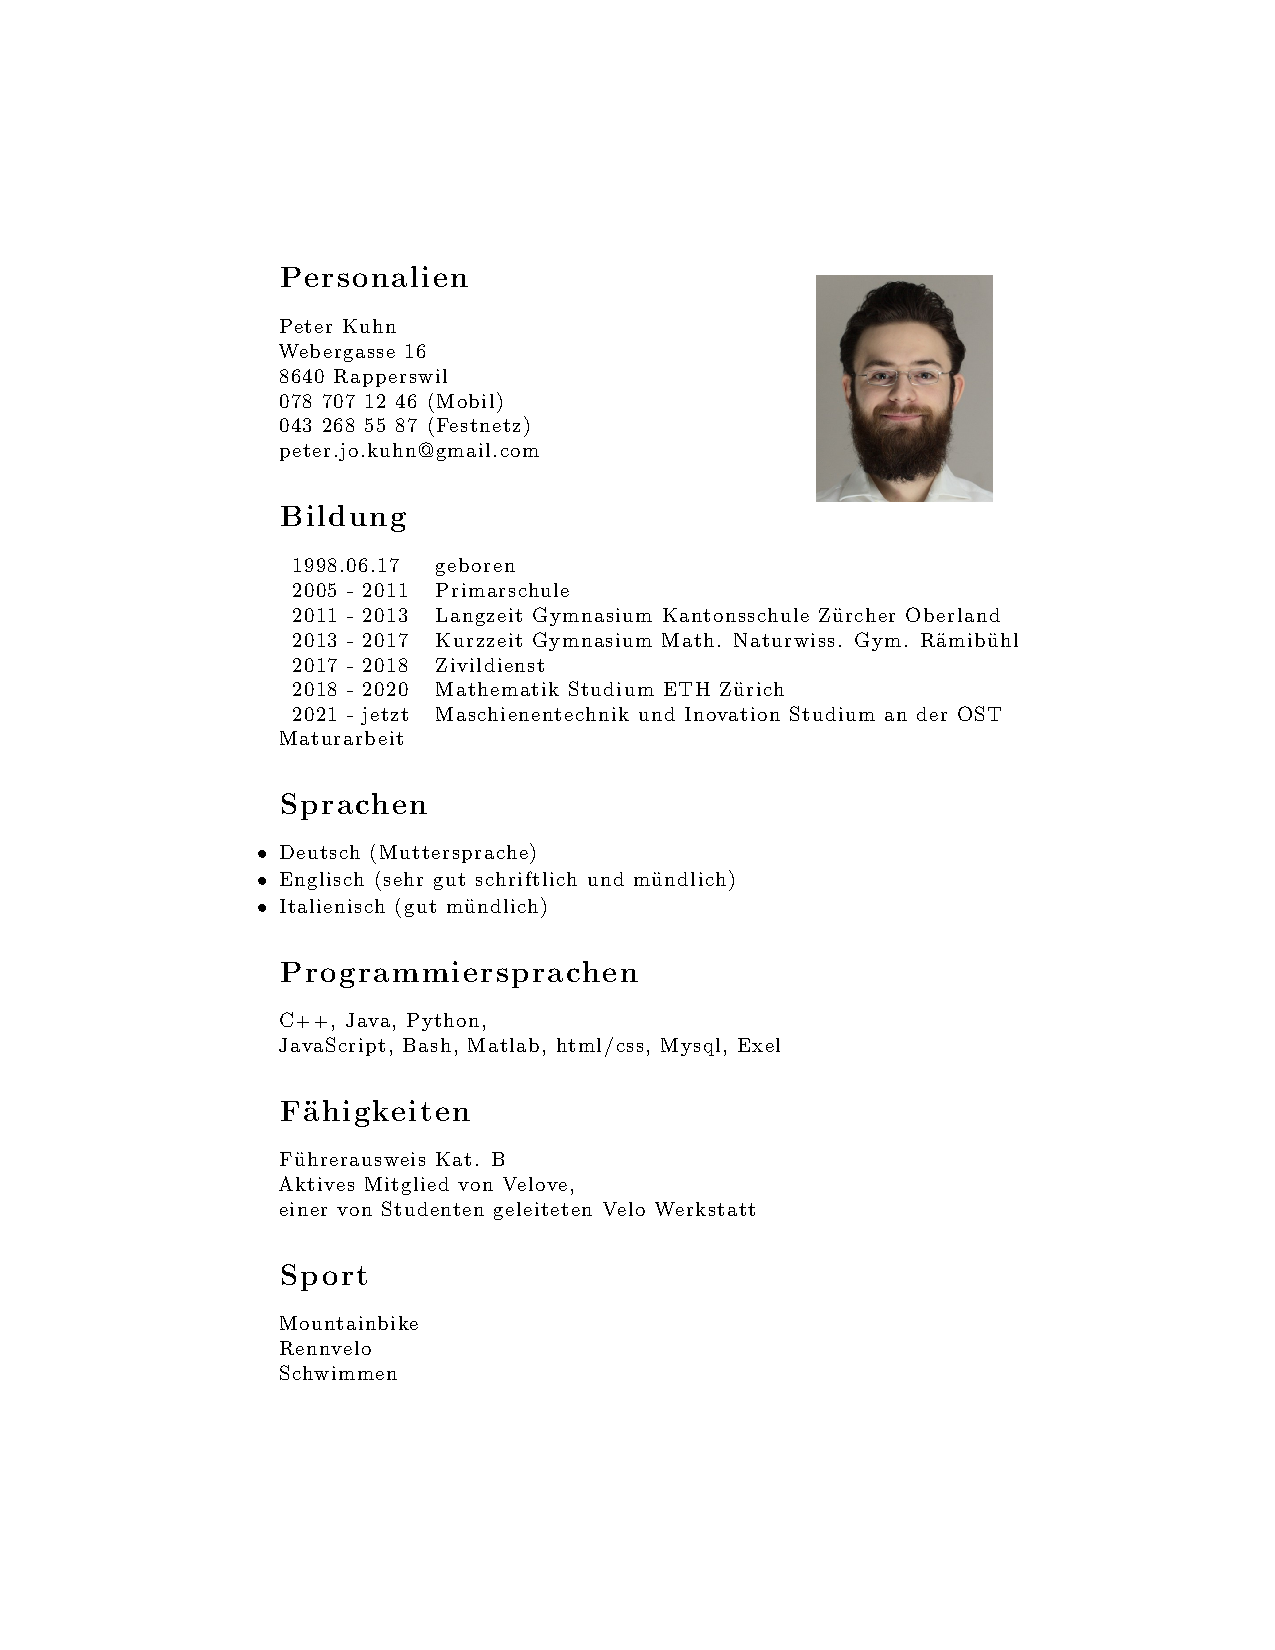
\includepdf{Bilder/lebenslauf-2.pdf}


\end{document}
